\chapter{彭庆福餐厅点单系统需求分析与概要设计}
本章对彭庆福餐厅点单系统进行了需求分析和概要设计,描述了系统设计目标、功能需求和非功能需求。介绍了系统总体设计与部署,通过数据库实体关系图解释了数据库设计。
\section{系统需求概述与可行性分析}
\subsection{系统设计目标}
彭庆福餐厅点单系统的核心目标是解决用户到店点餐、预约点餐、外卖点餐、付款、帮助与反馈等问题,同时为商家提供座位管理、菜品录入、库存预警、统计报表等功能。

本系统应该具有以下几个核心目标:
\begin{enumerate}
  \item 实现高效在线点单:系统提供到店、预约、外卖形式的点餐服务为顾客充分提供便利,节省排队点餐、等待上菜等时间,并为顾客自动保存购物车内已点菜品,保存外卖、预约点单的历史内容。
  \item 支持多角色点单:同一个顾客可能会有不同身份来用餐,比如工作时可以使用公司角色并享受相应的订单折扣,日常就餐可以使用个人角色,所以系统设置了多角色切换,允许用户使用所选角色进行点单。
  \item 到店用餐时,订单和座号相关联:顾客到店点餐时,将订单与座号绑定,顾客可以下单、加菜、取消订单、支付订单,只有当订单结束时,此座位才会转为开放状态,可以供下一位顾客使用。
  \item 实现在线支付结账:顾客不需要再去收银台结账,可以自行下单并且用支付宝、微信等方式支付订单。
  \item 较高问题解决率:系统有帮助与反馈入口,顾客可以提出意见与建议,系统会检索有无相关问题答案,如果有相关问题的答案,系统会快速反馈给顾客,如果没有,系统会发送给商家并在得到解答后返回给用户。
  \item 实现菜品信息录入:商家可以将菜品录入到每日要出品的发布中,使得顾客下单的时候可以及时看到当日菜品图片、名称以及其价格、份数等详情。
  \item 实现座位管理:商家可以录入餐厅位置实地信息,并登记座位,实时管理座位数、状态、是否拼单等信息。
  \item 实现库存管理:商家在采购需求中可以快速登记,录入当日所缺菜品,并且在生产实况中可以看到当前菜品空缺详情。
  \item 符合用户使用软件的习惯:顾客想点餐的时候需要方便快捷的渠道,而商家接单、处理订单一般在固定地点办公,所以系统将点单部分和管理部分分别设计成了包括微信公众号、支付宝和网页浏览在内的移动端和PC端,使得用户习惯该系统的使用方式。
\end{enumerate}

如图
~\ref{fig_strucCH3}所示,整个彭庆福餐厅点单系统由移动端、PC管理平台及后台服务器组成,顾客可以使用微信公众号、微信扫一扫、支付宝扫一扫或者Safari、IE、Chrome等浏览器以H5网页的形式接入到该系统,商家可以使用电脑以基于B/S模式的PC端网页的形式接入系统来管理菜品、订单等,后台服务器则为前端提供所需的各种接口服务~\cite{gzy}。
\begin{figure}[htbp!]
    \centering
    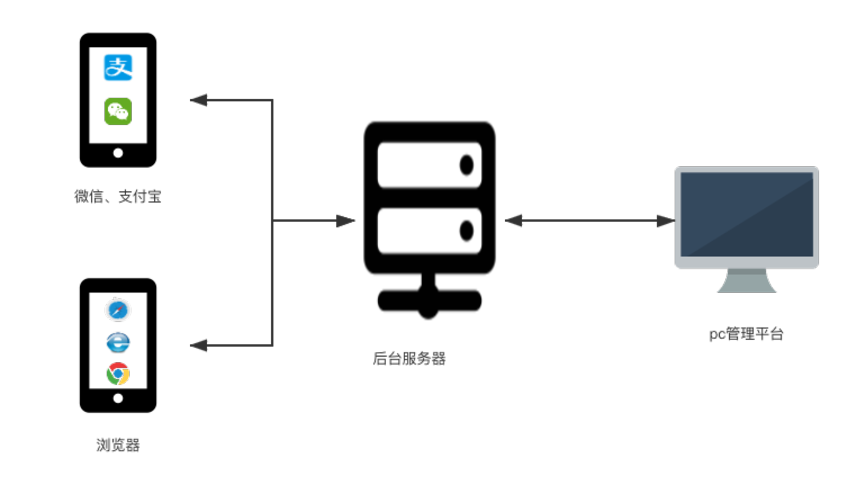
\includegraphics[width=5in]{FIGs/chapter3/struc.pdf}
    \caption{系统整体结构图}\label{fig_strucCH3}
\end{figure}

\subsection{需求概述}
为了满足顾客点餐时对于隐私的要求以及商家对点餐系统菜品溯源、订单管理与座位管理上的要求,本文设计了彭庆福餐厅点单系统,该系统从顾客和商家两方考虑,充分满足了二者对点单、管理上的需求,商家记录餐厅、菜品、座位、订单等信息,便于顾客查看餐厅详情、订单历史数据以及个人信息。
\begin{figure}[htbp!]
    \centering
    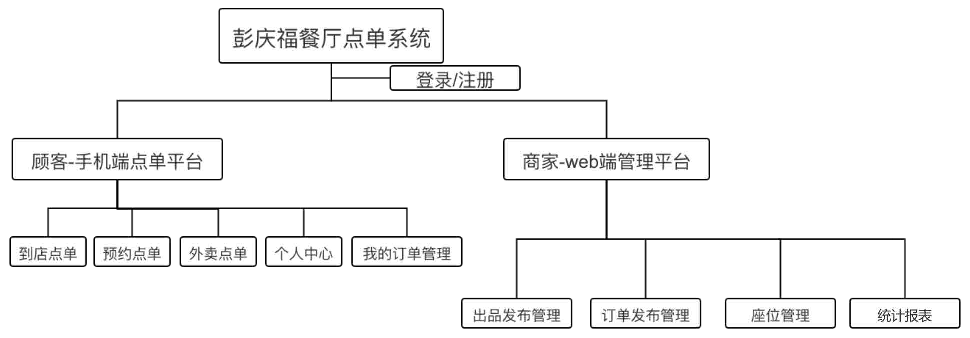
\includegraphics[width=5in]{FIGs/chapter3/function.pdf}
    \caption{系统功能需求结构图}\label{fig_functionCH3}
\end{figure}

如图
~\ref{fig_functionCH3}所示,彭庆福餐厅点单系统的入口有两种,一种是移动端包括浏览器、微信公众号以及支付宝扫码,需要实现顾客点单、支付、查看订单、修改个人信息;另一种是Web网页端,商家进行出品发布管理、订单发布管理、座位管理、菜品管理、统计报表等多种功能需求。

其中,顾客可以通过到店扫码、关注微信公众号、浏览器直接输入地址等方式进入平台,登录注册后实现到店、预约、外卖点单等操作。商家可以通过Web地址从电脑网站直接进入平台进行管理,实现从注册商家到登记菜品、创建座位仓库、创建出品发布、管理订单发布、管理座位信息、管理菜品等操作。\\

\subsection{可行性分析}
技术可行性:后端采用传统的Spring MVC框架加上Spring Cloud微服务部署架构与Spring Boot技术的结合,这类开发技术已经比较完善、成熟,可供参考的技术资料比较充足,可以对接分布式发布订阅消息系统Kafka进行数据流方面的处理。前端采用的React与Redux框架比较稳定且易上手,UI方面使用蚂蚁金服设计的比较成熟的Ant Design达到视觉上美观、统一的效果。因此,本系统的可行性非常高。

经济可行性:随着国民经济的不断提升以及互联网的飞速发展,人们对于饮食方面的需求越来越多样化,对隐私的要求也越来越高,传统的点单系统已经无法满足多样化需求,急需一款可以保护用户隐私,帮助顾客推荐喜好、查看历史操作、查看菜品原料从采摘到售卖的历史记录,帮助商家进行库存管理、报表分析、订单管理等操作的新型点单系统。彭庆福餐厅点单系统为实现这些需求应运而生,具有良好的发展前景。该系统上手难度小,参考代码模板多,并且已经与餐厅提前沟通好宣传方案,其开发成本、推广成本都比较低,具有比较高的经济效益前景。

\section{系统需求分析}
\begin{table}[htbp!]\footnotesize
  \centering
  \caption{彭庆福餐厅点单系统的主要功能需求列表}
  \vspace{2mm}
  \begin{tabular}{clp{0.6\columnwidth}}
  \toprule
  \textbf{需求编号}&\textbf{需求名称}&\textbf{需求描述}\\
  \midrule 
  \textbf{R1}& 到店点单& 顾客到店后,扫描桌子上二维码点单就餐,可以在线选购菜品、加菜、退菜、取消订单、付款。\\
  \hline
  \textbf{R2}& 预约点单& 若餐厅未在营业时间内,顾客可以手机预约点单,填写用餐时间、人数、电话后,在线预约下单,并在该时间段去店内就餐。\\
  \hline
  \textbf{R3}& 外卖点单& 顾客可以随时随地在手机上进行外卖点单,填写收货地址、配送时间、联系姓名、联系电话以及人数后,在线下单外卖等待配送。\\
  \hline
  \textbf{R4}& 个人中心& 顾客可以在个人中心查看个人状态、更改角色、退出登录,在帮助与反馈栏中提出意见等。\\
  \hline
  \textbf{R5}& 我的订单管理& 顾客可以打开我的订单,查看订单列表,可点击具体订单查看订单详情、支付订单,可以对未完成订单进行退菜、加菜、取消订单等操作。\\
  \hline
  \textbf{R6}& 出品发布管理& 商家可以每日创建一个出品发布,来设置当天餐厅营业时间段、菜品管理(包括菜品类别管理、增删改菜品)、查看采购需求、进行菜品的快速登记。\\
  \hline
  \textbf{R7}& 订单发布管理& 当顾客手机下单后,商家可以查看到当前餐厅的所有订单列表,可对订单进行删改,点击进入相应订单查看详情,进行取消菜品、结算、确认顾客离店、打印订单等操作。\\
  \hline
  \textbf{R8}& 座位管理& 商家可以设置餐厅开放时间,多视图(卡片视图、平面视图、时间轴视图)管理座位仓库,座位设置成功后会有和每个座位相对应的二维码,可以对座位及二维码信息进行管理。\\
  \hline
  \textbf{R9}& 统计报表& 商家点击报表查看每日、每月的收支报表、菜品进销存报表,可以根据时间筛选查看或打印任意日期的报表内容。\\
  \bottomrule
  \end{tabular}
  \label{table:requireList}
\end{table}

该系统涉众主要两种,分别是顾客和商家。不同的用户角色对于该系统有如下需求~\cite{lb2009}:

\begin{enumerate}
    \item 顾客:顾客随时随地都有可能点单,并且在系统使用过程中可能会遇到一系列自己无法解决的问题,他们需要一个方便、快捷的平台,可以快速而准确地满足其饮食需求。最佳方式就是注册并登录该系统,将所需菜品直接选购下单完成付款。
    \item 商家:商家一般是熟悉餐厅运营,了解菜品详情、每日库存与订单详情的员工,对菜品销售非常熟悉并且有固定的办公场地。他们需要一个系统来统计菜品销售和库存,处理顾客的各种订单与问题,录入当日菜品数量、更新库存等。
  \end{enumerate}

通过以上分析可以得出如表~\ref{table:requireList}所示的彭庆福餐厅点单系统的部分主要功能需求,以下分别从顾客和商家角度对该系统功能需求作出具体分析。\\

\subsection{顾客功能需求}
顾客功能需求部分是彭庆福餐厅点单系统中主要由手机操作的部分,其用例图如图
~\ref{fig_customerCH3}所示,主要包括了到店点单、预约点单、外卖点单、个人中心、我的订单管理等功能,其具体包含功能如下:
\begin{figure}[htbp!]
  \centering
  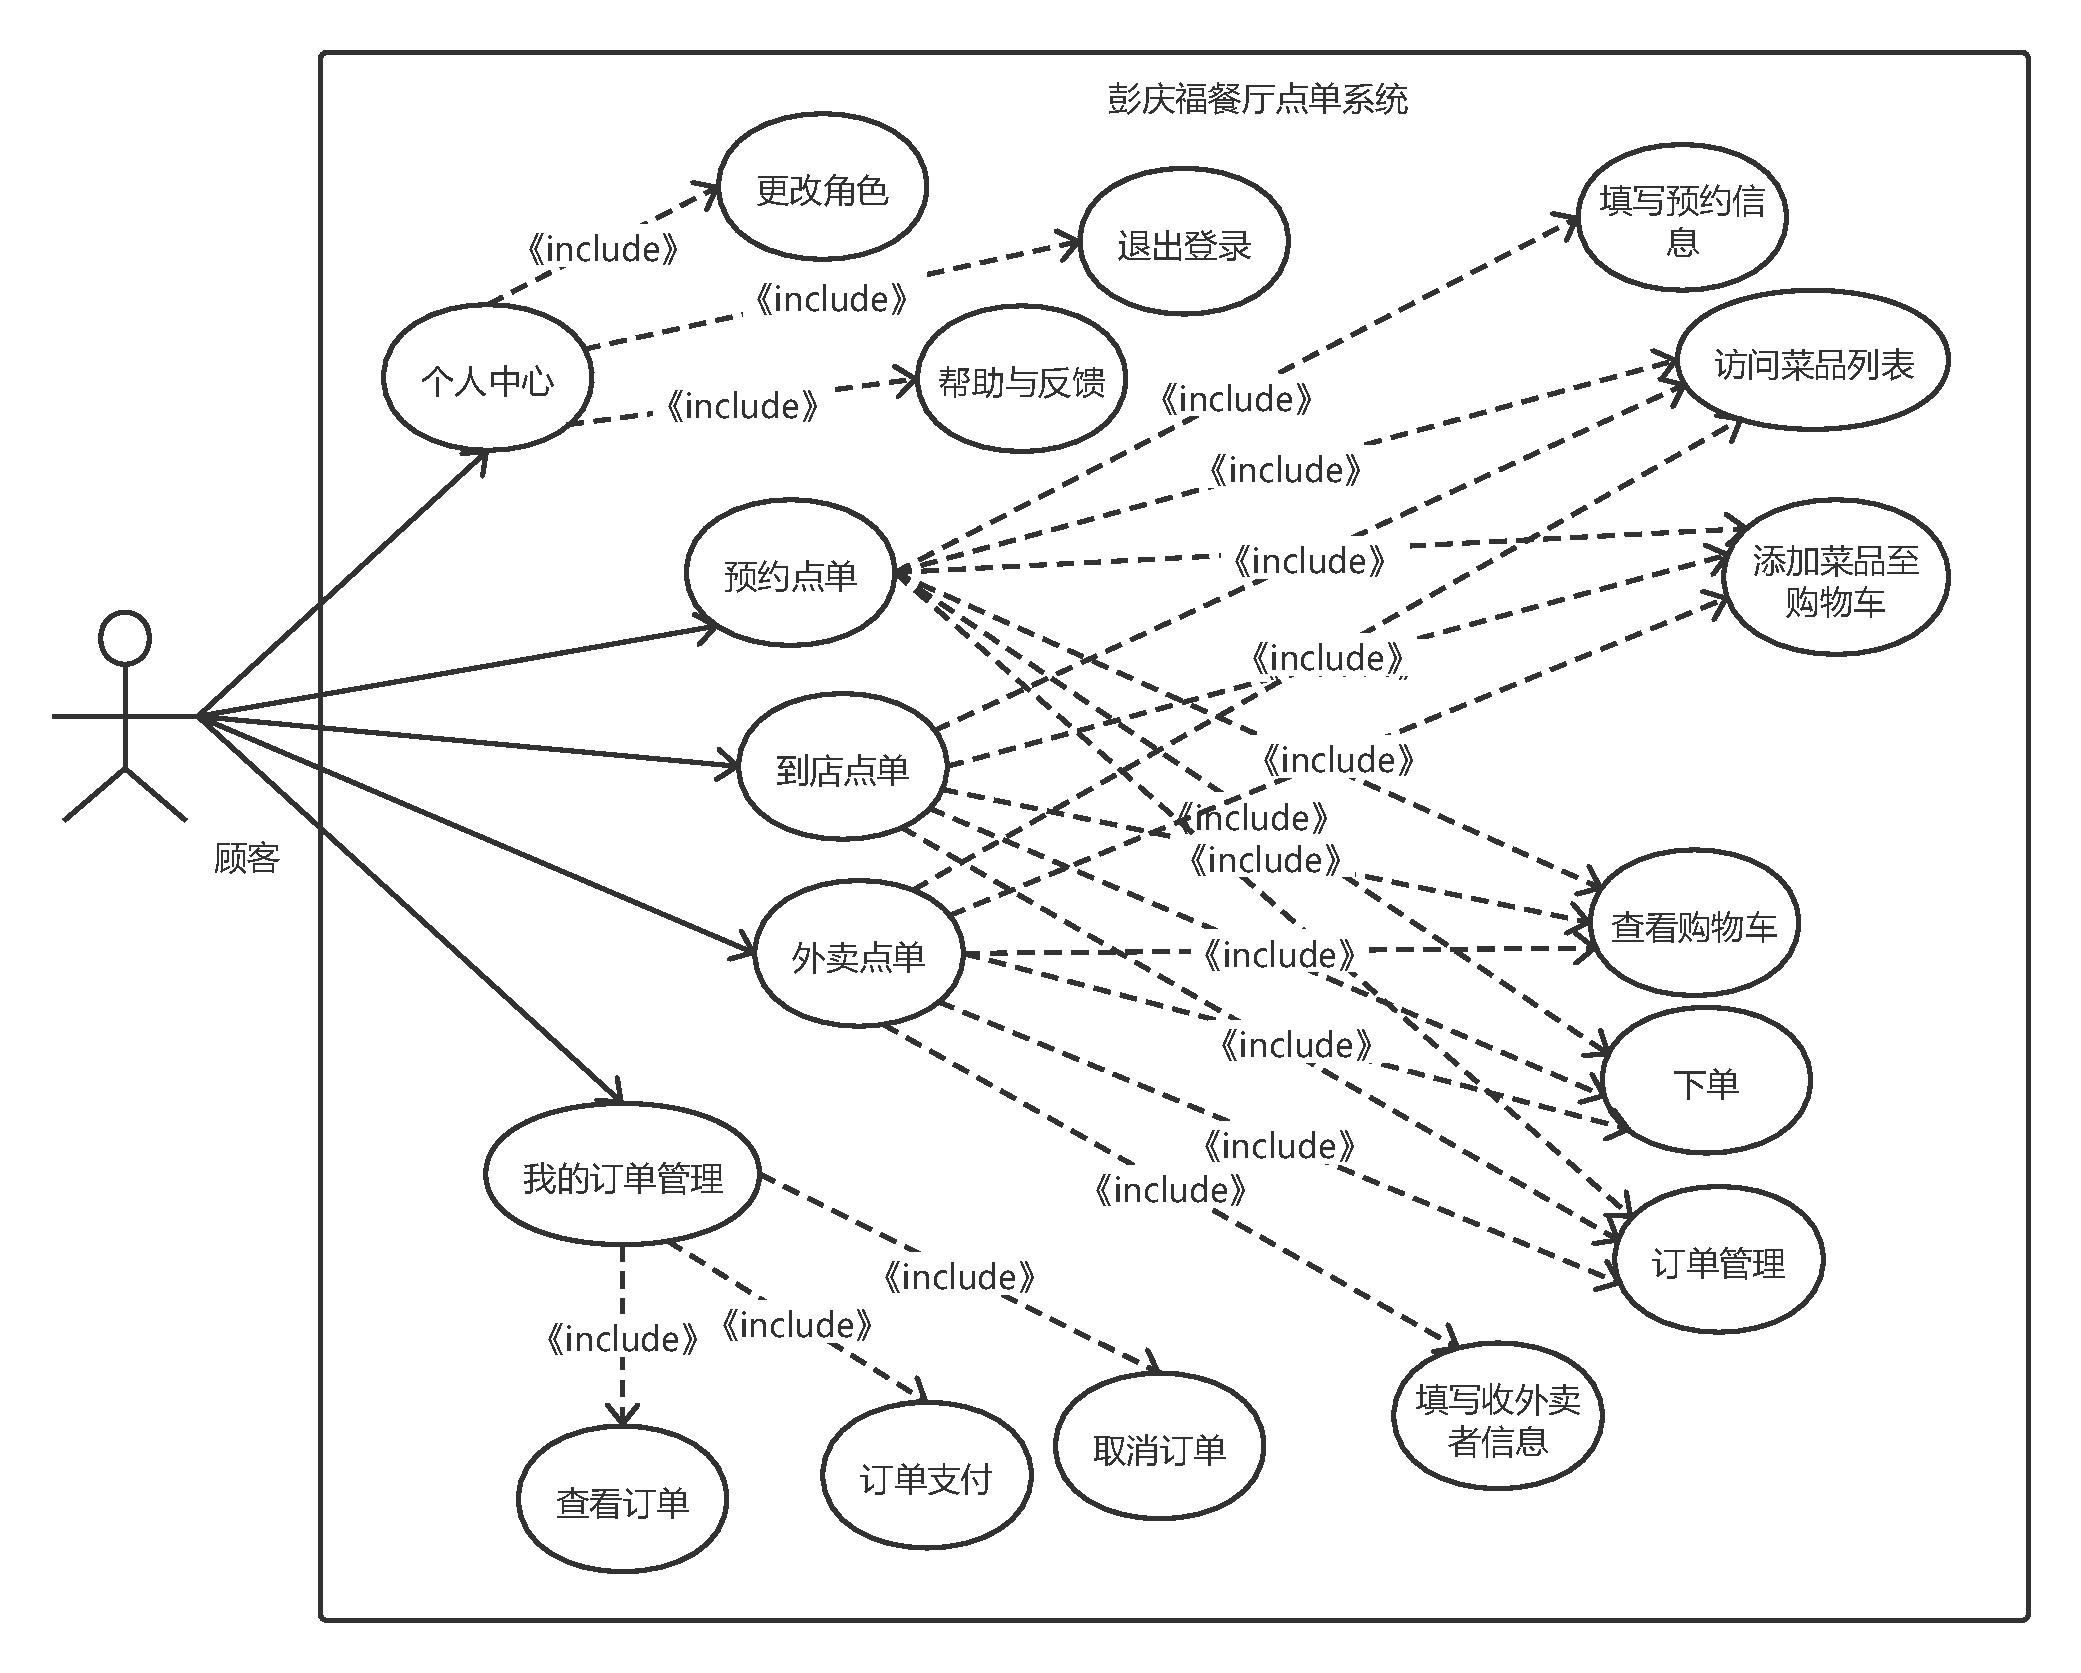
\includegraphics[width=5in]{FIGs/chapter3/customer.pdf}
  \caption{顾客就餐模块用例图}\label{fig_customerCH3}
\end{figure}

下面将详细描述关于顾客点单平台的几个重要用例~\cite{ymh}。

如表~\ref{table:uc1}所示,其描述了顾客到店点单的具体过程,顾客在成功登录系统后点击店内就餐可以选定座位并扫描桌上二维码进行点菜、增删所选菜品数量、查看购物车、下单等操作。用户到店点单时,需要扫描座位上的二维码才能进行下单,如果该座位当前已经有订单,系统会提醒顾客,并且判断座位的当前订单是否为该用户订单,如果是则提示跳转到该订单详情页,如果不是则提醒用户该座位已有订单,需要换一个座位下单。

顾客预约点单与之类似,未在餐厅营业时间时或者想要提前预约之后时间来就餐,顾客可以选择提前预约点菜下单,在指定时间就餐或者在此之前取消菜品即可。系统考虑到顾客隐私安全问题,在账号登录时需要用户认证,付款时也需要二次认证保护顾客付款的安全性。顾客将部分菜品加入购物车后,不小心退出点单界面,之后再次进入时,系统会记录顾客历史操作,保留购物车内菜品,方便顾客继续点单。

\begin{table}[htbp!]
  \footnotesize
  \centering
  \caption{到店点单用例表}
  \vspace{2mm}
  \begin{tabular}{cp{11.5cm}}
   \hline
   \ ID & UC1 \\ 
   \hline
   \ 名称 & 到店点单 \\ 
   \hline
   \ 参与者 & 顾客,目标是根据个人需要创建一个菜品订单。 \\ 
   \hline
   \ 优先级 & 高 \\ 
   \hline
   \ 触发条件 & 用户需要在餐厅内用餐。 \\ 
   \hline
   \ 前置条件 & 用户成功登录彭庆福餐厅点单系统,并拥有点单权限。 \\ 
   \hline
   \ 后置条件 & 菜品订单创建成功,用户成功用餐。 \\ 
   \hline
   \multirow{2}{*}{正常流程}
    & 1.	已成功登录的用户进入主页,点击店内就餐。\\
    & 2.	系统按照不同类别显示该餐厅当日所有菜品。\\
    & 3.	用户扫描座位上二维码。\\
    & 4.	系统显示相应座位号。\\
    & 5.	用户选择就餐角色、就餐时间、就餐人数以及菜品种类和数量,点击下单。\\
    & 6.	系统提示下单成功,并展示订单详情。\\
    & 7.	用户查看详情并选择相应操作。\\
    & 8.  系统保存用户修改并更新界面。 \\
   \hline
   \multirow{2}{*}{扩展流程}
    & 3a. 未在商家营业时间:\\
    & ~~1.	系统提示未在营业时间,接受预约,用户无需扫码。\\
    & ~~2.	返回步骤5。\\
    & 3b. 该用户当前有未完成的到店订单:\\
    & ~~1.	系统提示用户还有未完成订单,并跳转到相应订单详情页面。\\
    & 3c. 该座位当前有未完成的订单,且不是该用户的:\\
    & ~~1.	系统提示用户该座位已有订单,提示其更换座位下单。\\
    & ~~2.	返回步骤2。\\
    & 7a. 用户选择加菜:\\
    & ~~1.	系统返回菜单页面供用户添加菜品并下单。\\
    & 7b. 用户选择相应菜品退菜:\\
    & ~~1.	系统保存更改并更新订单详情页面(退掉的菜品不会再显示)。\\
    & 7c. 用户选择取消订单:\\
    & ~~1.  系统保存更改并更新订单详情页面(订单状态变成已取消)。\\
  \hline
  \ 特殊需求 & 无 \\ 
  \hline
  \end{tabular}
  \label{table:uc1}
\end{table}

如下表~\ref{table:uc2}所示,其描述了顾客外卖点单的具体过程,顾客在成功登录系统后点击外卖点餐可以选择地址,填写收外卖者信息,进行点菜、增删所选菜品及修改其数量、查看购物车、下单等操作。顾客可以在操作的任意步骤内返回上一页面进行内容修改,系统会保存顾客操作,提高可用性。由于到店点单、预约点单与座位相关联,所以一个用户同一时刻只能有一个正在进行的相关订单,但是外卖订单可以同时下单多个,根据顾客需要送至相同或不同地址。

此操作可以帮助顾客随时随地点单,系统会默认记录收外卖者信息,使得下次点单时不需要再重新录入个人信息。外卖点单的选择地址组件引用了高德地图API的React组件——React-AMap,不光自动定位当前位置,顾客还可以自由定位所在位置或者搜索选定某一位置作为接收地点,系统会判断外卖是否在商家配送范围内并进行相应提醒。在商家确认订单之前,顾客可以选择取消订单,并且可以随时查看订单状态,跟踪骑手位置,有效帮助顾客了解订单详情,提升其就餐满意度。
\begin{table}[htbp!]
  \footnotesize
  \centering
  \caption{外卖点单用例表}
  \vspace{2mm}
  \begin{tabular}{cp{11.5cm}}
   \hline
   \ ID & UC3 \\ 
   \hline
   \ 名称 & 外卖点单 \\ 
   \hline
   \ 参与者 & 顾客,目标是根据个人需要创建外卖订单。 \\ 
   \hline
   \ 优先级 & 高 \\ 
   \hline
   \ 触发条件 & 用户需要外卖用餐。 \\ 
   \hline
   \ 前置条件 & 用户成功登录彭庆福餐厅点单系统,并拥有点单权限。 \\ 
   \hline
   \ 后置条件 & 外卖订单创建成功,用户成功用餐。 \\ 
   \hline
   \multirow{2}{*}{正常流程}
    & 1.	已成功登录的用户进入主页,点击外卖点餐。\\
    & 2.	系统显示需要用户填写的内容。\\
    & 3.	用户选择收货地址、配送时间,填写联系姓名、联系电话、人数。\\
    & 4.	用户填写完毕,点击确认并点餐。\\
    & 5.	系统按照不同类别显示该餐厅当日所有菜品。\\
    & 6.	用户选择菜品种类和数量,点击下单。\\
    & 7.	系统显示包括菜品种类、数量以及收外卖者信息和合计价格。\\
    & 8.	用户点击确认并选择付款方式付款。\\
    & 9.  系统提示下单成功,并展示订单详情。 \\
    & 10.	用户点击取消订单。\\
    & 11.  系统保存用户修改并更新界面,订单状态变成已取消。 \\
    & 用户可以重复步骤3-11,直至完成所有要下单的外卖内容。\\
   \hline
   \multirow{2}{*}{扩展流程}
    & 3a. 用户发现信息填写有误,选择返回:\\
    & ~~1.	返回步骤2。\\
    & 3b. 用户搜索地址相关字:\\
    & ~~1.	系统返回相关地址内容供用户选择。\\
    & 7a. 用户发现菜品选择有误,选择返回:\\
    & ~~1.	返回步骤5。\\
  \hline
  \ 特殊需求 & 无 \\ 
  \hline
  \end{tabular}
  \label{table:uc2}
\end{table}

如下表~\ref{table:uc3}所示,其描述了顾客管理个人中心的具体过程,顾客在成功登录系统后点击个人头像可以进入个人中心,该界面会显示当前所选角色、头像,以及用户账号等基本信息。顾客可以选择切换角色、提出意见与建议、退出登录等操作,并得到相应的反馈内容。

顾客在该页面下可以清晰看到个人信息,并且可以更换不同角色进行不同操作与查看。每个角色对应现实生活中的一种身份,比如个人角色、公司角色等,也会有与之对应的操作权限与折扣优惠。

顾客如果对软件或是餐厅有任何问题需要解决,都可以点击“帮助与反馈”按钮,填写问题详情点击提交,问题会很快反映给商家,待其解决会将反馈以消息形式推送给顾客供其查看。顾客也可以选择退出登录,则系统会将其安全退出,并跳转到登录注册页面。

\begin{table}[htbp!]
  \footnotesize
  \centering
  \caption{个人中心用例表}
  \vspace{2mm}
  \begin{tabular}{cp{11.5cm}}
   \hline
   \ ID & UC4 \\ 
   \hline
   \ 名称 & 个人中心 \\ 
   \hline
   \ 参与者 & 顾客,目标是查看并管理个人信息。 \\ 
   \hline
   \ 优先级 & 中 \\ 
   \hline
   \ 触发条件 & 用户需要管理个人信息。 \\ 
   \hline
   \ 前置条件 & 用户成功登录彭庆福餐厅点单系统。 \\ 
   \hline
   \ 后置条件 & 个人信息修改成功。 \\ 
   \hline
   \multirow{2}{*}{正常流程}
    & 1.	已成功登录的用户点击个人头像进入个人中心界面。\\
    & 2.	系统显示当前用户头像、账号以及当前角色。\\
    & 3.	用户查看详情并进行相应操作。\\
    & 4.	系统保存用户修改并更新界面。\\
    & 用户可以重复步骤3、4,直至完成所有要操作的内容。\\
   \hline
   \multirow{2}{*}{扩展流程}
    & 3a. 用户点击当前角色:\\
    & ~~1.	系统显示当前用户的所有角色。\\
    & ~~2.	用户选择想要切换的角色。\\
    & 3b. 用户点击帮助与反馈:\\
    & ~~1.	系统显示帮助与反馈界面。\\
    & ~~2.	用户输入问题,点击提交。\\
    & 3c. 用户点击退出登录:\\
    & ~~1.	系统退出当前账户。\\
    & ~~2.	系统跳转到登录界面。\\
  \hline
  \ 特殊需求 & 无 \\ 
  \hline
  \end{tabular}
  \label{table:uc3}
\end{table}

如下表~\ref{table:uc4}所示,其描述了顾客进行订单管理的具体过程,顾客在成功登录系统后点击我的订单可以查看所有历史订单记录,选择某一具体订单点击查看详情并进行管理~\cite{zh2015}。

根据顾客所选角色,会显示相应的订单列表。顾客可以根据已完成(包括待评价、已评价、已取消等状态)、未完成(包括待付款、用餐中、配送中等状态)、全部(包括已完成、未完成的所有状态)这三种可选择类型来查看个人历史订单,可以点击某订单,查看订单详情,并根据订单状态进行相应可操作内容,比如待付款订单可以进行取消订单、付款、加菜、退菜等操作;用餐中订单可以对未出餐的菜品进行取消等操作;已结束的订单可以对单个菜品或是本次用餐进行评价等操作,系统会根据用户操作进行相应页面更新、提示与响应。

\begin{table}[htbp!]
  \footnotesize
  \centering
  \caption{我的订单管理用例表}
  \vspace{2mm}
  \begin{tabular}{cp{11.5cm}}
   \hline
   \ ID & UC5 \\ 
   \hline
   \ 名称 & 我的订单管理 \\ 
   \hline
   \ 参与者 & 顾客,目标是查看我的订单并管理。 \\ 
   \hline
   \ 优先级 & 高 \\ 
   \hline
   \ 触发条件 & 用户需要查看我的订单。 \\ 
   \hline
   \ 前置条件 & 用户成功登录彭庆福餐厅点单系统,并拥有查看我的订单权限。 \\ 
   \hline
   \ 后置条件 & 我的订单查看完成。 \\ 
   \hline
   \multirow{2}{*}{正常流程}
    & 1.	已成功登录的用户进入主页,点击我的订单。\\
    & 2.	系统根据全部、未完成、已完成三种状态显示订单列表。\\
    & 3.	用户点击某一订单。\\
    & 4.	系统显示该订单详情。\\
    & 5.  用户查看详情并进行相应操作。\\
    & 6.  系统保存用户修改并更新界面。\\
    & 用户可以重复步骤3-6,直至完成所有要操作的规则。\\
   \hline
   \multirow{2}{*}{扩展流程}
    & 5a. 若当前订单商家还未确认,且非外卖订单:\\
    & ~~1.	用户选择加菜。\\
    & ~~2.	系统返回菜单页面供用户添加菜品并下单。\\
    & ~~3.	用户选择相应菜品退菜。\\
    & ~~4.	系统保存更改并更新订单详情页面(退掉的菜品不会再显示)。\\
    & ~~5.	用户选择取消订单。\\
    & ~~6.	系统保存更改并更新订单详情页面(订单状态变成已取消)。\\
    & ~~7.	用户选择支付。\\
    & ~~8.	系统根据当前操作环境和用户选择的付款方式显示相应付款界面。\\
    & 5b. 若当前订单商家还未确认,且订单类型是外卖:\\
    & ~~1.	用户点击取消订单。\\
    & ~~2.	系统保存用户修改并更新界面(订单状态变成已取消)。\\
    & 5c. 若当前订单已结束还未评价:\\
    & ~~1.	用户点击相应菜品进行评价,对本次用餐进行评价。\\
    & ~~2.	系统保存用户修改并更新界面(订单状态变成已评价)。\\
  \hline
  \ 特殊需求 & 无 \\ 
  \hline
  \end{tabular}
  \label{table:uc4}
\end{table}
\subsection{商家功能需求}
\begin{figure}[htbp!]
  \centering
  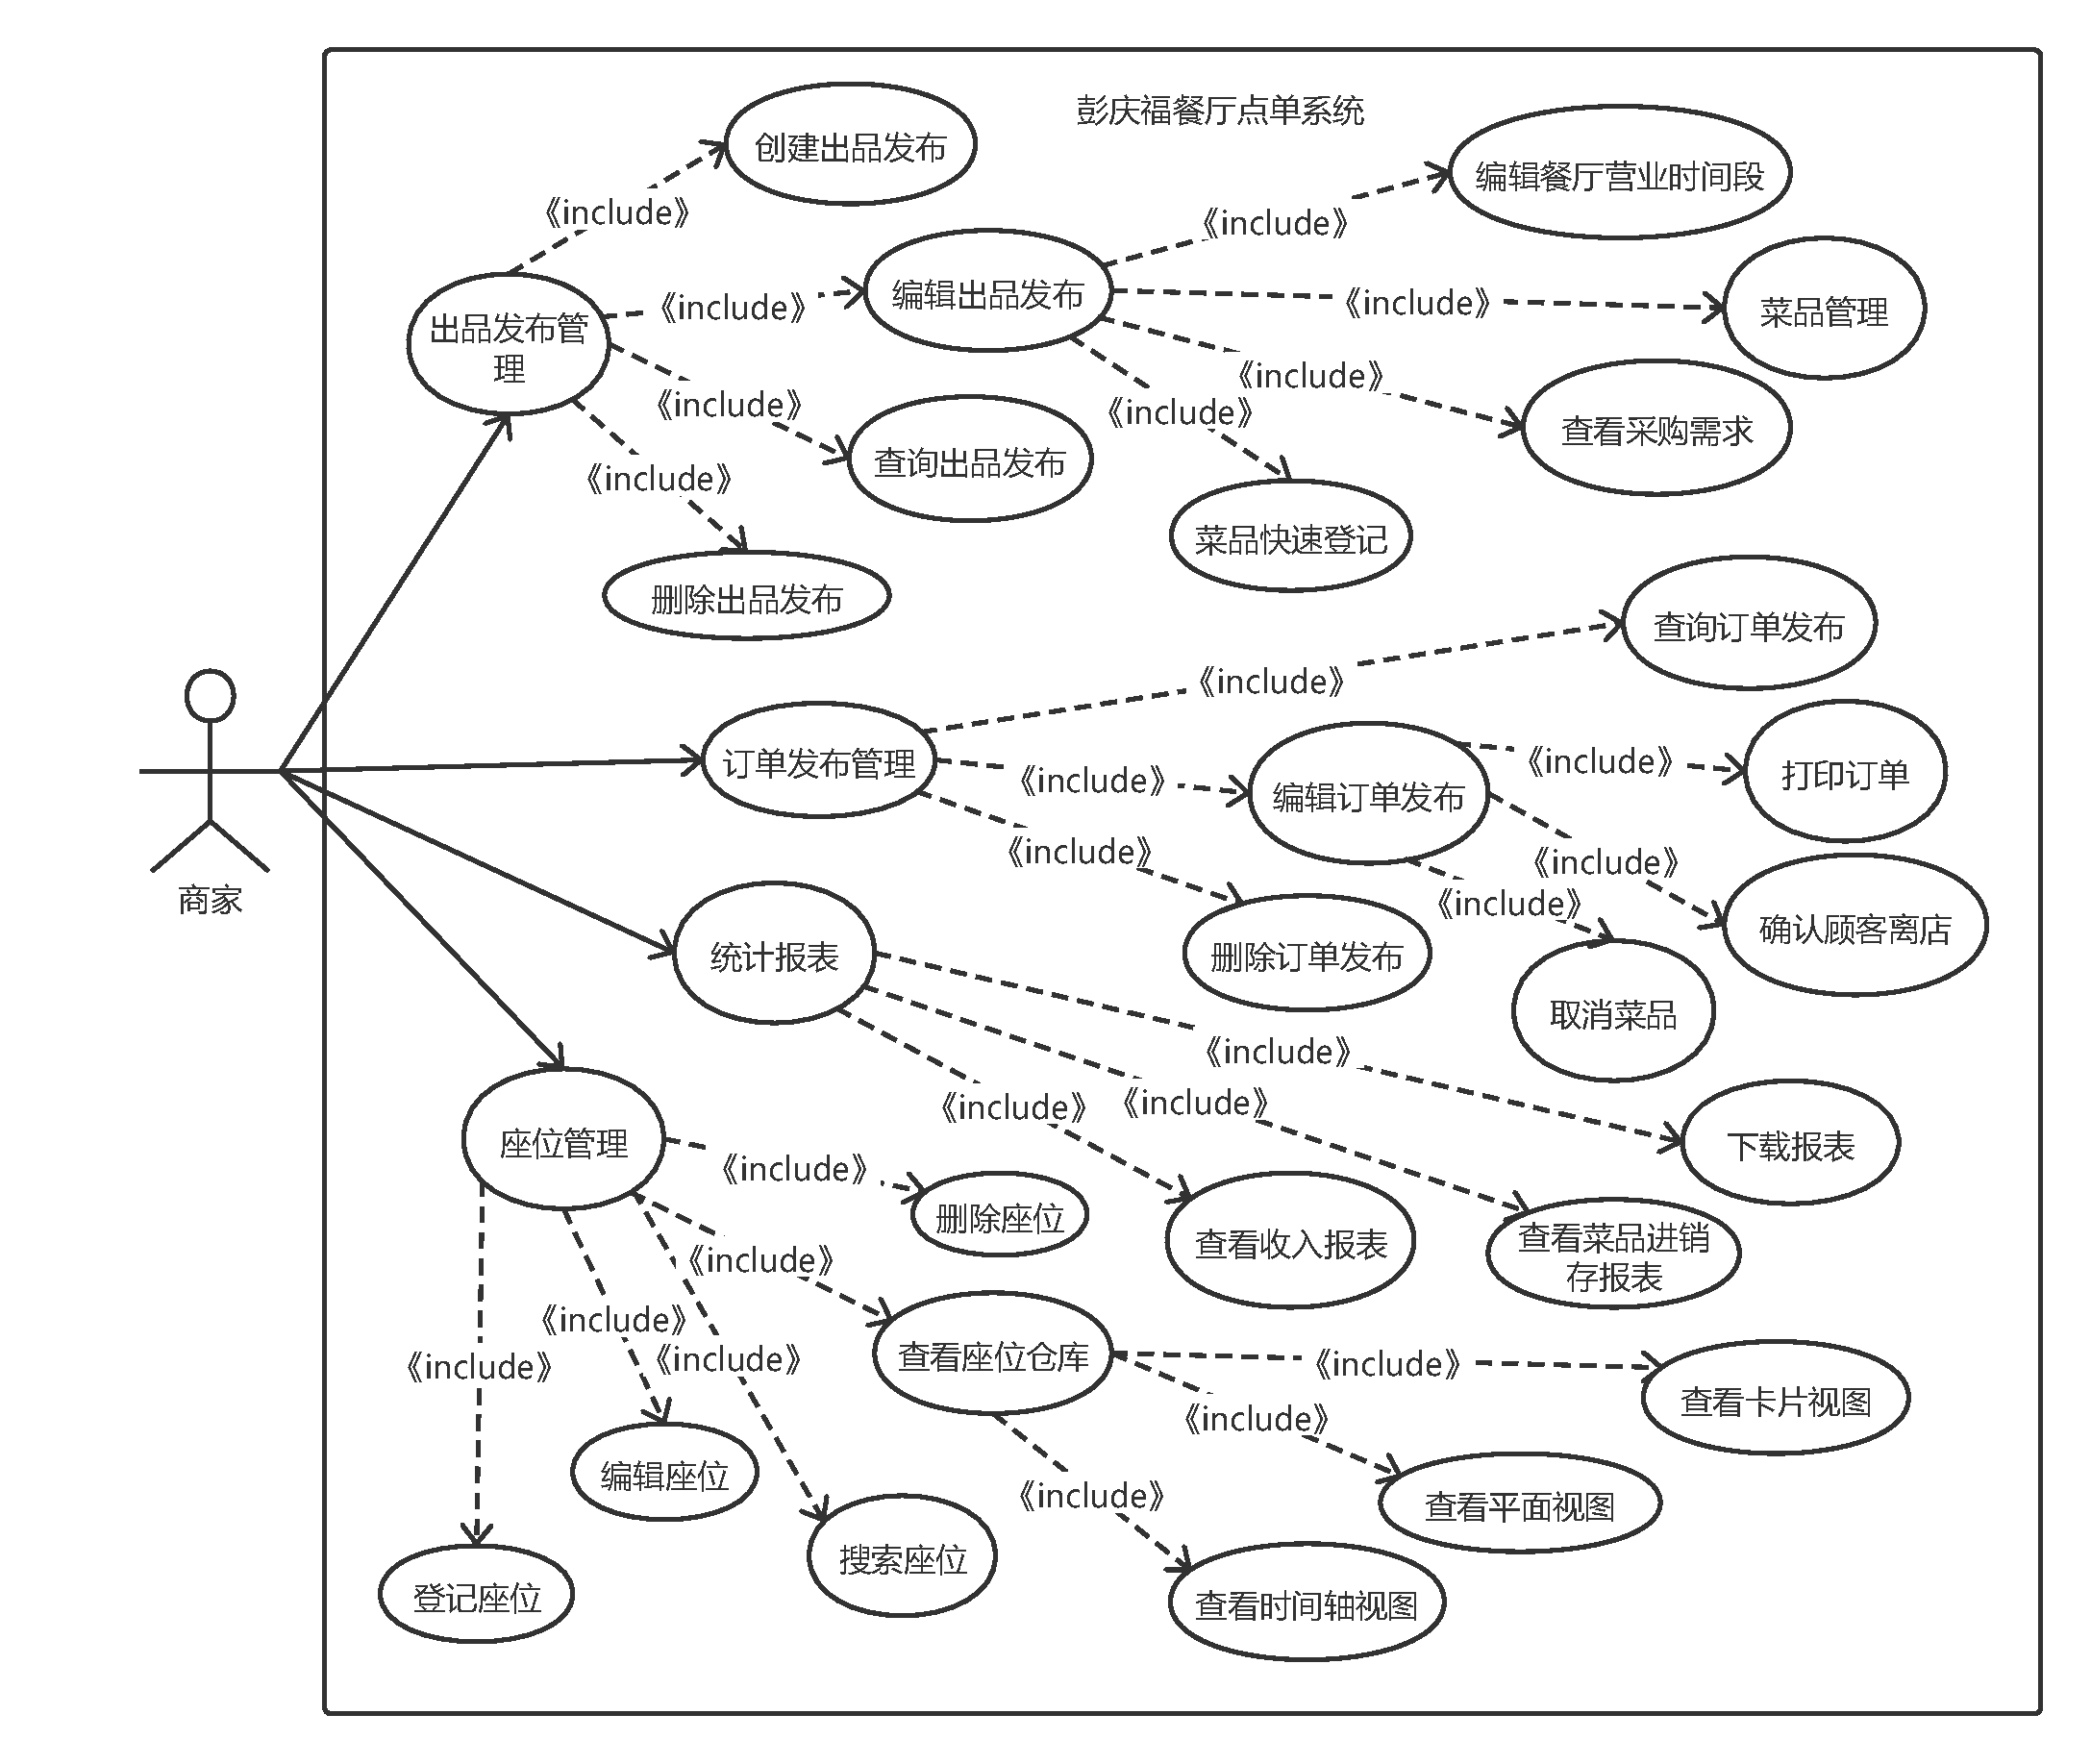
\includegraphics[width=5in]{FIGs/chapter3/seller.pdf}
  \caption{商家管理模块用例图}\label{fig_sellerCH3}
\end{figure}

商家功能需求部分,是彭庆福餐厅点单系统中主要由Web端网页操作的部分~\cite{yzl2017},其用例图如图~\ref{fig_sellerCH3}所示,主要包括了出品发布管理、订单发布管理、座位管理、统计报表等功能,商家成功登录系统后,可以根据需要进行不同的操作来管理、运营餐厅。

下面将详细描述关于商家管理平台的几个重要用例。

如表~\ref{table:uc5}所示,其描述了商家对出品发布管理的具体过程,出品发布由商家创建,它包含每日计划营业时间段、对菜品的分类管理、对库存的增补管理等。商家在成功登录系统后点击筛选发布中的出品发布,可以看到餐厅历史所有的出品发布列表,可以根据需要创建新的出品发布,设置餐厅每日的营业时间、菜单等。可以根据需要搜索筛选特定的出品发布,点击某一出品发布标题,可以查看该出品发布的详情并进行管理更新。

对于创建好的出品计划,商家可以进行查看,包括出品时间、当日的营业时间段、要出售的产品、计划份数、订单份数等;也可以进行相应管理,包括更新餐厅当日的营业时间段,可以添加、修改、删除多段时间,增删改当日要销售的菜品(包括单个菜品、套餐等);也可以查看采购需求,根据库存提示进行相应的库存补充。商家将需要修改的发布内容都修改完成后,点击“更新出品发布”按钮,发布才会更新,这样帮助商家减少误操作,避免引发不必要的错误,相当于二次确认。创建新的出品发布时,可以复用已有的出品发布内容,只需要修改出品日期,系统会自动记录复用的出品发布内容并进行复用,商家可以在原有的内容基础上进行更新。

\begin{table}[htbp!]
  \footnotesize
  \centering
  \caption{出品发布管理用例表}
  \vspace{2mm}
  \begin{tabular}{cp{11.5cm}}
   \hline
   \ ID & UC6 \\ 
   \hline
   \ 名称 & 出品发布管理 \\ 
   \hline
   \ 参与者 & 商家,目标是查看并管理所有出品发布。 \\ 
   \hline
   \ 优先级 & 高 \\ 
   \hline
   \ 触发条件 & 用户需要查看餐厅的所有出品发布。 \\ 
   \hline
   \ 前置条件 & 用户成功登录彭庆福餐厅点单系统,并拥有管理出品发布的权限。 \\ 
   \hline
   \ 后置条件 & 出品发布列表内容更新。 \\ 
   \hline
   \multirow{2}{*}{正常流程}
    & 1.	已成功登录的用户进入发布页面,点击出品发布。\\
    & 2.	系统显示餐厅所有的出品发布列表。\\
    & 3.	用户输入出品发布关键字,选择搜索。\\
    & 4.	系统显示与之相关的出品发布。\\
    & 5.  用户点击某一出品发布。\\
    & 6.  系统显示该出品发布详情。\\
    & 7.  用户查看详情,并选择相应操作。\\
    & 8.  系统保存用户修改并更新界面。\\
    & 用户可以重复步骤3-8,直至完成所有要搜索、查询和修改的出品发布。\\
   \hline
   \multirow{2}{*}{扩展流程}
    & 3a. 用户选择添加出品发布,并输入内容:\\
    & ~~1.	若填写内容有误,系统提示正确格式。\\
    & ~~2.	填写无误,用户点击确定后,系统保存更改并更新出品发布列表。\\
    & 4a. 要查询的出品发布不存在:\\
    & ~~1.	系统提示该出品发布不存在。\\
    & 7a. 用户选择编辑出品发布,并填写修改内容:\\
    & ~~1.	用户修改餐厅当日营业时间段,系统保存更改并更新界面。\\
    & ~~2.	用户对当日菜品做修改,增删菜品,系统保存更改并更新界面。\\
    & ~~3.	用户查看采购需求,并对当日库存不足的菜品进行快速登记,系统保存更改并更新界面。\\
    & 7b. 用户选择删除该出品发布:\\
    & ~~1.	系统请用户再次确认,确认成功后系统删除该出品发布并更新界面内容。\\
    & ~~2.	再次确认时用户选择取消,系统不做更改,返回详情界面。\\
  \hline
  \ 特殊需求 & 无 \\ 
  \hline
  \end{tabular}
  \label{table:uc5}
\end{table}

如下表~\ref{table:uc6}所示,其描述了商家对订单发布进行管理的具体过程,订单发布由系统自动创建。有顾客下单时,订单发布就会新增一条订单与之对应,它包含订单号、座位、就餐人数、顾客用餐时间、到店时间以及订单的菜品详情、总金额等。商家在成功登录系统后,点击筛选发布中的订单发布就可以看到餐厅历史所有的订单发布列表,点击具体订单发布查看订单发布详情并进行管理。

商家进入某个订单详情页面后,可以看到订单类型、状态、订单号、座位、顾客用餐时间等顾客信息和所点菜品信息,根据订单状态以及个人权限进行相应操作,比如修改订单的就餐人数。对于已经支付的订单,商家可以点击确认离店结束订单状态,可以查看订单的相应评论、个人评论,回复顾客评论。

\begin{table}[htbp!]
  \footnotesize
  \centering
  \caption{订单发布管理用例表}
  \vspace{2mm}
  \begin{tabular}{cp{11.5cm}}
   \hline
   \ ID & UC7 \\ 
   \hline
   \ 名称 & 订单发布管理 \\ 
   \hline
   \ 参与者 & 商家,目标是查看并管理所有订单发布。 \\ 
   \hline
   \ 优先级 & 高 \\ 
   \hline
   \ 触发条件 & 用户需要查看餐厅的所有订单发布。 \\ 
   \hline
   \ 前置条件 & 用户成功登录彭庆福餐厅点单系统,并拥有管理订单发布的权限。 \\ 
   \hline
   \ 后置条件 & 订单发布列表内容更新。 \\ 
   \hline
   \multirow{2}{*}{正常流程}
    & 1.	已成功登录的用户进入发布页面,点击订单发布。\\
    & 2.	系统显示餐厅所有的订单发布列表。\\
    & 3.	用户输入订单发布关键字,选择搜索。\\
    & 4.	系统显示与之相关的订单发布。\\
    & 5.  用户点击某一订单发布。\\
    & 6.  系统显示该订单发布详情。\\
    & 7.  用户查看详情,并选择相应操作。\\
    & 8.  系统保存用户修改并更新界面。\\
    & 用户可以重复步骤3-8,直至完成所有要搜索、查询和修改的订单发布。\\
   \hline
   \multirow{2}{*}{扩展流程}
    & 4a. 要查询的订单发布不存在:\\
    & ~~1.	系统提示该订单发布不存在。\\
    & 7a. 用户选择编辑订单发布,并填写修改内容:\\
    & ~~1.	用户打印订单详情,系统打印出包含菜品信息及金额的账单。\\
    & ~~2.	用户取消订单内某菜品,系统保存更改并更新界面。\\
    & ~~3.	当顾客用餐完成且订单状态为已支付时,用户点击确认离店,系统保存更改并更新界面。\\
    & 7b. 用户选择删除该订单发布:\\
    & ~~1.	系统请用户再次确认,确认成功后系统删除该订单发布并更新界面内容。\\
    & ~~2.	再次确实时用户选择取消,系统不做更改,返回详情界面。\\
  \hline
  \ 特殊需求 & 无 \\ 
  \hline
  \end{tabular}
  \label{table:uc6}
\end{table}

如下表~\ref{table:uc7}所示,其描述了商家对座位管理的具体过程,商家在成功登录系统后,点击座位库可以查看所有座位~\cite{zdx2019},选择不同视图进行座位列表查看,点击具体座位可以查看详情并进行管理。

\begin{table}[htbp!]
  \footnotesize
  \centering
  \caption{座位管理用例表}
  \vspace{2mm}
  \begin{tabular}{cp{11.5cm}}
   \hline
   \ ID & UC8 \\ 
   \hline
   \ 名称 & 座位管理 \\ 
   \hline
   \ 参与者 & 商家,目标是查看并管理所有座位。 \\ 
   \hline
   \ 优先级 & 高 \\ 
   \hline
   \ 触发条件 & 用户需要查看餐厅的所有座位。 \\ 
   \hline
   \ 前置条件 & 用户成功登录彭庆福餐厅点单系统,并拥有管理座位的权限。 \\ 
   \hline
   \ 后置条件 & 座位库内容更新。 \\ 
   \hline
   \multirow{2}{*}{正常流程}
    & 1.	已成功登录的用户进入座位库。\\
    & 2.	系统显示座位库内的所有座位。\\
    & 3.	用户选择不同的视图查看。\\
    & 4.	系统根据选择显示不同视图的座位列表。\\
    & 5.  用户输入关键字,选择搜索。\\
    & 6.  系统显示所有相关的座位。\\
    & 7.  用户点击登记座位,填写座位编号、座位数、座位类型,并确认。\\
    & 8.  系统保存内容,并更新座位库。\\
    & 9.	用户点击某座位删除。\\
    & 10.	系统保存内容,并更新座位库。\\
    & 11.  用户点击某一座位。\\
    & 12.  系统显示该座位详情,包括座号、二维码、状态、座位数、类型以及占用情况记录。\\
    & 13.  用户查看详情,并选择相应操作。\\
    & 14.  系统保存用户修改并更新界面。\\
    & 用户可以重复步骤3-14,直至完成所有要操作的规则。\\
   \hline
   \multirow{2}{*}{扩展流程}
    & 3a. 用户选择时间轴视图:\\
    & ~~1.	系统显示当天各个座位被占用的时刻图,用户可以筛选时间查看不同日期座位的时间轴视图。\\
    & ~~2.	用户点击某个座位的某状态下的时间块。\\
    & ~~3.	系统跳转到相关的订单发布详情页面。\\
    & 3b. 用户选择平面视图:\\
    & ~~1.	系统显示各个座位在地图上的坐标信息,用户可以编辑平面视图,管理地图上各个座位的相关信息。\\
    & 3c. 用户选择卡片视图:\\
    & ~~1.	系统显示当天各个座位基本信息,用户可以查看座位信息、设置座位状态。\\
    & 5a. 搜索座位不存在:\\
    & ~~1.	系统提示该座位不存在。\\
    & 7a. 若填写内容有误:\\
    & ~~1.	系统显示错误,并提示正确格式。\\
    & 13a. 用户选择下载二维码:\\
    & ~~1.	系统下载该座位的二维码到本地。\\
    & 13b. 用户筛选不同日期:\\
    & ~~1.	系统根据日期显示该座位的占用情况记录。\\
  \hline
  \ 特殊需求 & 无 \\ 
  \hline
  \end{tabular}
  \label{table:uc7}
\end{table}

商家可以从三种不同的视图来查看和管理座位库。

默认视图为卡片视图,可以看到座位列表以卡片形式呈现,商家可以根据座号、座位状态、时间来组合筛选座位,可以修改座位状态,进行座位的增删改,也可以点击座位详情进行查看具体信息。商家可以选择时间轴视图,查看不同日期的餐厅座位被预订、占用以及空闲状态,可以在相应的状态上点击进入到相关的订单发布中查看具体的订单详情。商家也可以选择平面视图,编辑座位或者餐厅的实际地址信息,在高德地图或者自己上传的餐厅平面图上进行打点、画圈,将地理位置与座位卡片相关联。

\begin{table}[htbp!]
  \footnotesize
  \centering
  \caption{统计报表用例表}
  \vspace{2mm}
  \begin{tabular}{cp{11.5cm}}
   \hline
   \ ID & UC9 \\ 
   \hline
   \ 名称 & 统计报表 \\ 
   \hline
   \ 参与者 & 商家,目标是统计报表。 \\ 
   \hline
   \ 优先级 & 高 \\ 
   \hline
   \ 触发条件 & 用户需要查看餐厅收入、菜品进销存的报表。 \\ 
   \hline
   \ 前置条件 & 用户成功登录彭庆福餐厅点单系统,并拥有统计报表的权限。 \\ 
   \hline
   \ 后置条件 & 统计报表内容更新。 \\ 
   \hline
   \multirow{2}{*}{正常流程}
    & 1.	已成功登录的用户进入统计报表页面。\\
    & 2.	系统显示当日收入报表。\\
    & 3.	用户点击菜品进销存报表。\\
    & 4.	系统显示当日进销存报表。\\
    & 5.  用户点击下载报表。\\
    & 6.  系统下载当前报表。\\
    & 用户可以重复步骤3-6,直至完成所有要操作的规则。\\
   \hline
   \multirow{2}{*}{扩展流程}
    & 3a. 用户选择不同时间筛选:\\
    & ~~1.	系统根据时间显示不同的报表。\\
  \hline
  \ 特殊需求 & 无 \\ 
  \hline
  \end{tabular}
  \label{table:uc8}
\end{table}

如表~\ref{table:uc8}所示,其描述了商家统计报表的具体过程,商家在成功登录系统后,点击统计报表查看收入报表和菜品进销存报表,点击下载可以保存报表。\\

\subsection{系统非功能性需求分析}
\begin{table}[htbp!]
  \footnotesize
  \centering
  \caption{非功能性需求表}
  \vspace{2mm}
  % l - left, r - right, c - center. | means one vertical line
  \begin{tabular}{cp{9.5cm}}
  % \midrule
  \hline
  \multirow{3}{3.5cm}{
    \textbf{可用性}
    }&1. 为符合用户的正常操作习惯,将不同类型操作分开,不同用户群体的使用端分开。\\
    &2. 系统需要在用户完成某些操作后给出对应消息提醒,比如提示弹窗、二次确认弹框等。\\
    &3. 系统在必要情况下需提供使用帮助文档或者说明页面,使用户在使用系统时可以降低操作难度。\\
  \hline
  \multirow{2}{3.5cm}{
    \textbf{系统性能}
    }&1. 系统在同一时间内响应需要超过190个请求。\\
    &2. 系统能在用户操作时间的0.4秒内提供其相应反馈。\\
  \hline
  \multirow{2}{3.5cm}{
    \textbf{支持性}
    }&系统能在Windows、Mac OS、Linux等主流操作系统上运行,并且能在手机端正常使用,在微信客户端、支付宝客户端以及主流浏览器(比如IE、Chrome、Opera、Safari等)上良好运行。\\
  \hline
  \multirow{2}{3.5cm}{
    \textbf{可靠性}
    }&服务器有可能会宕机,需要在多台服务器中部署服务,使得某台服务器宕机后,服务依然可以正常使用。\\
  \hline
  \multirow{2}{3.5cm}{
    \textbf{安全性}
    }&1. 系统需要确保用户个人资料的安全性,其中包含用户密码、电话、个人基本情况等。\\
    &2. 系统通过权限管理来控制用户权限,使得不同类型用户的操作权限可以不同。\\
  \hline
  \end{tabular}
  \label{table:systemsRequirement}
\end{table}
如表~\ref{table:systemsRequirement}所示,是系统对非功能性需求的要求,包括可用性、系统性能、支持性、可靠性以及安全性。

\section{顾客功能执行流程设计}
设计该系统是为了能够高效、便捷解决顾客在日常生活中因为用餐产生的各种问题,也是为了商家能够节省时间,准确定位到每一个订单,更好地统计菜品种类库存、顾客历史订单等数据~\cite{zss2018}。

\begin{figure}[htbp!]
  \centering
  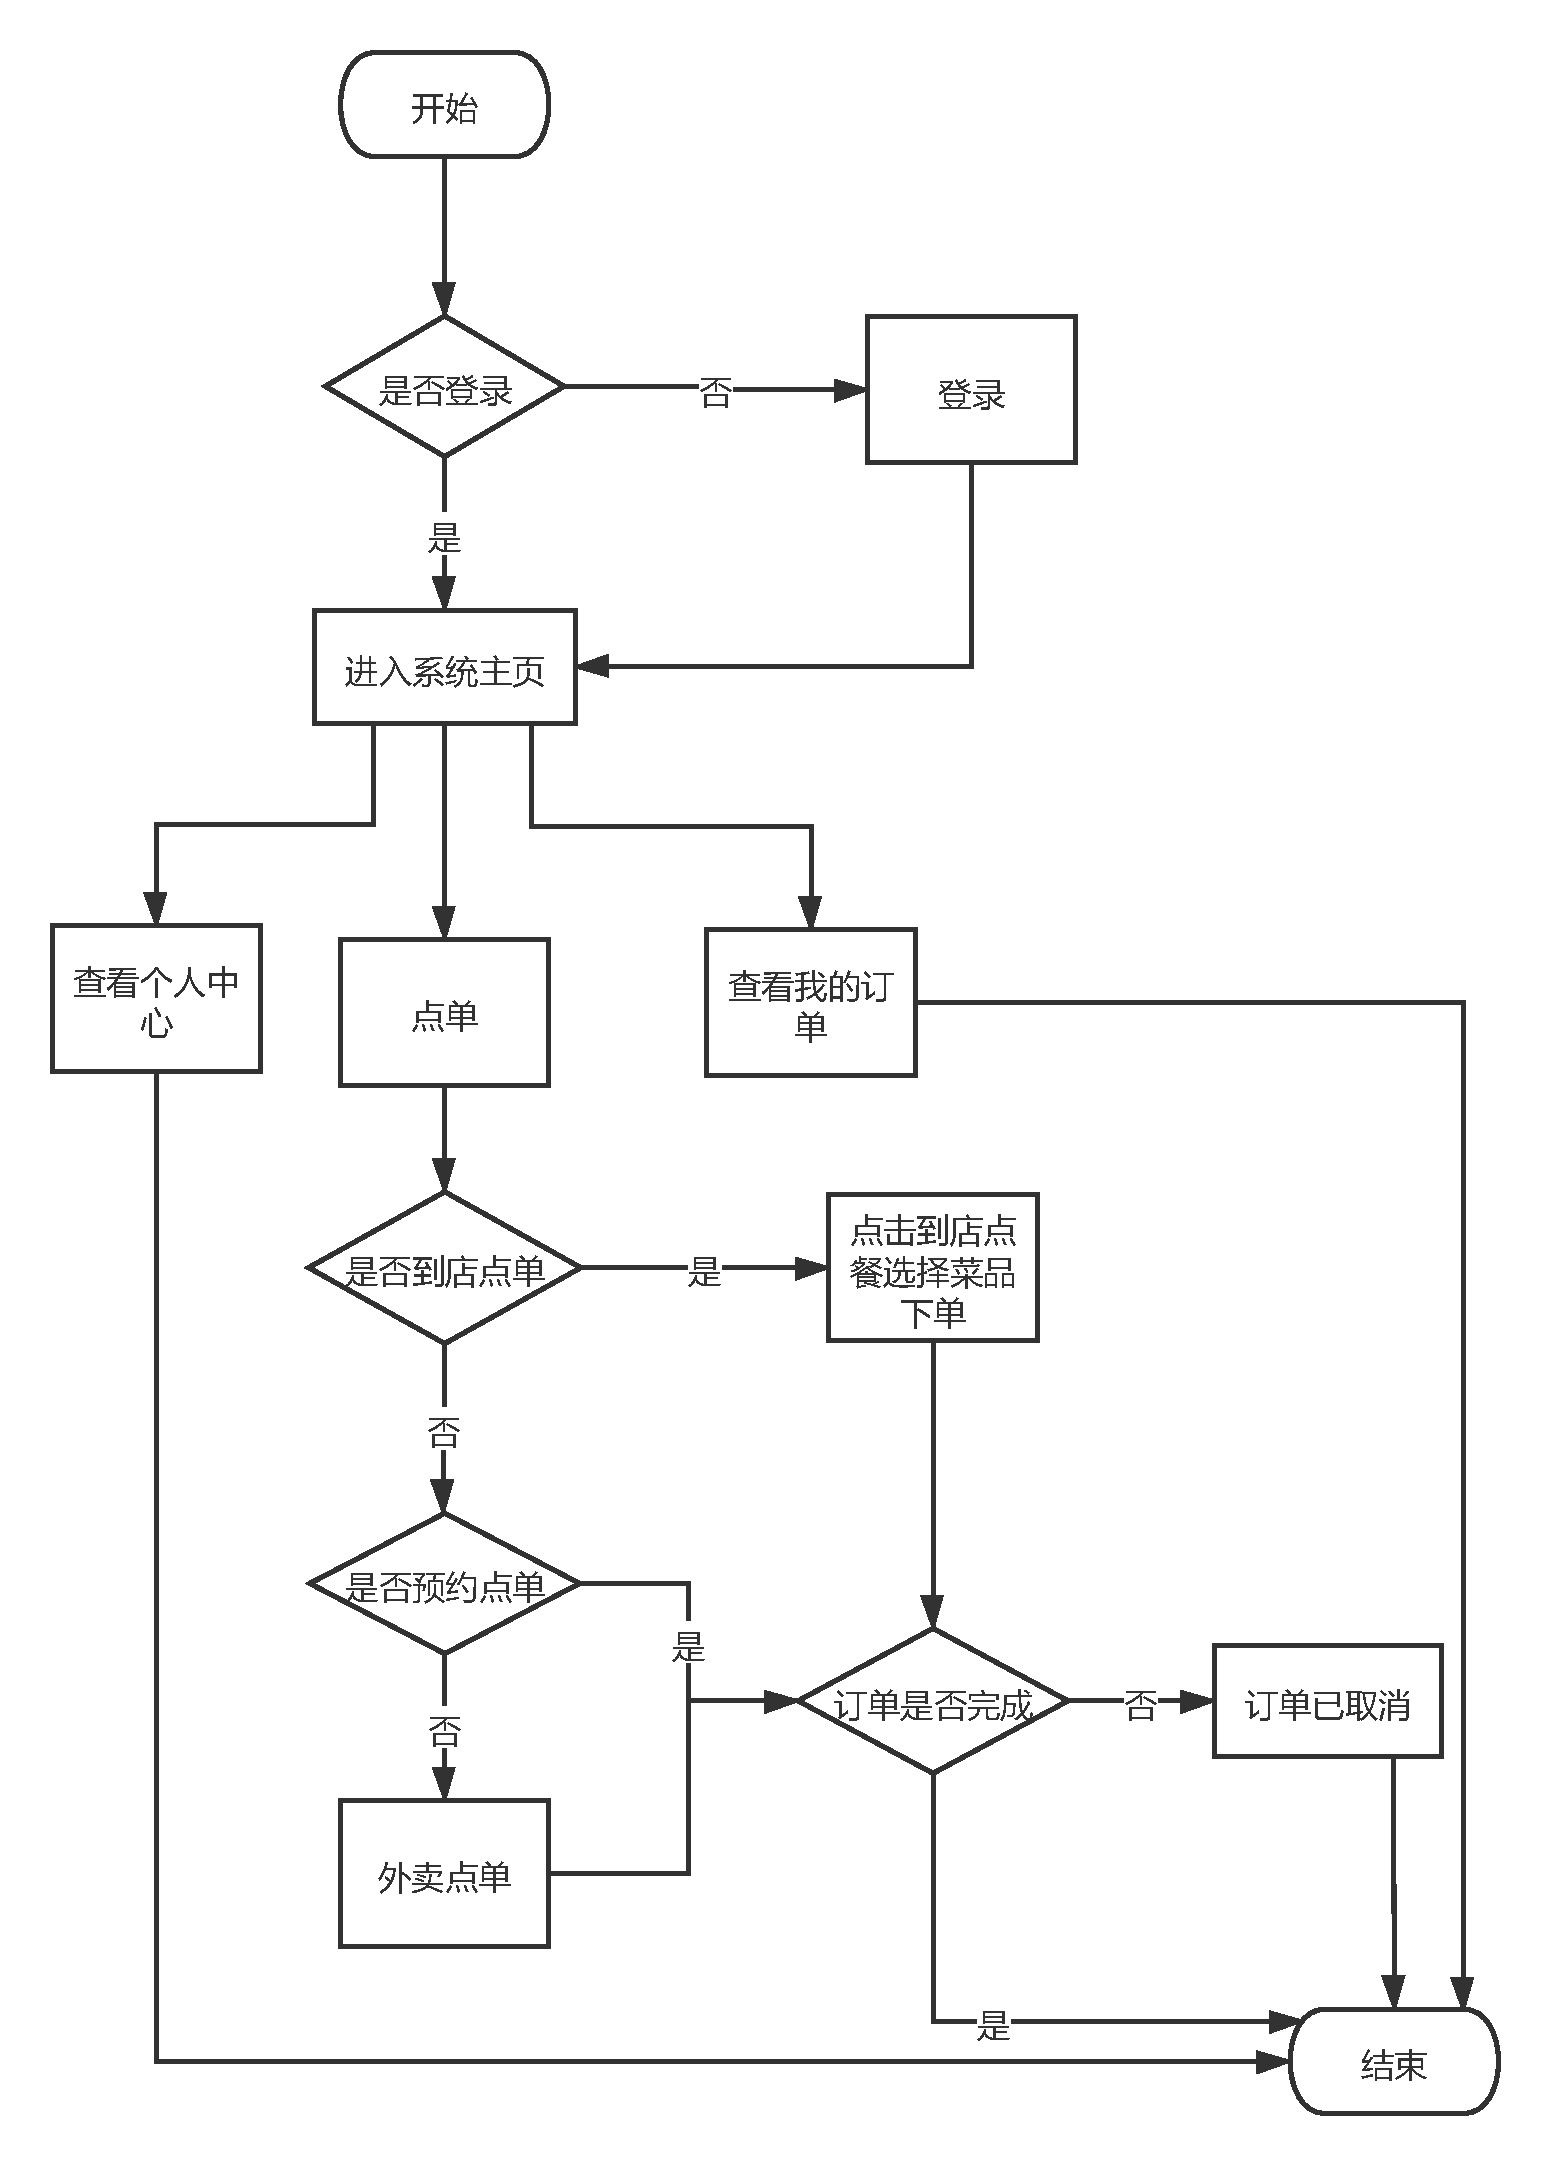
\includegraphics[width=4in]{FIGs/chapter3/flow.pdf}
  \caption{顾客主页功能的执行流程图}\label{fig_flowCH3}
\end{figure}

如图~\ref{fig_flowCH3}所示,这是顾客访问系统的主要执行流程图,以下对该图进行详细描述~\cite{liu2014design}:
\begin{enumerate}
  \item 顾客首先进入系统主页,如果没有登录则跳转到登录页面。
  \item 系统提供点单、查看个人中心、查看我的订单功能,顾客可以选择查看信息,若只是查看信息则查看完成后结束整个流程,若要点单则转向步骤3。
  \item 顾客是否在餐厅运营期间且已经到店进行点餐,若是则可扫码座位上二维码下单,如果不是则可以预约点单或者外卖点单。
  \item 如果订单完成或者取消则结束整个流程。
\end{enumerate}

\section{系统概要设计}
本节主要介绍了彭庆福餐厅点单系统的总体设计、系统部署、数据库设计等信息。\\
\subsection{总体设计}
该系统中,顾客可以通过关注商家的微信公众号,使用公众号内自定义的菜单栏进入系统,也可以使用支付宝、浏览器扫一扫座位号进入点单页面~\cite{swain2019electrical}。顾客点单页面使用HTML5页面展示,商家在PC端设置店铺状态、菜品管理以及订单管理,系统部署在服务器集群上,有五台服务器分工服务,实现负载均衡。为了使用户在高并发环境下也可以正常进行点单、下单等操作,保证良好的用户体验,系统使用了分布式缓存Redis存储用户一般经常访问的数据内容,以减轻查询数据库的压力~\cite{zcy2013redis}。商家会实时获取到用户下单的各个类型订单,以便及时准备菜品并送达,系统采用云平台在消息队列中存储订单,监听云打印机的在线情况方便实时打印用户订单。

系统的支付功能采用新型支付方式——移动支付,其中包括微信、支付宝支付,用户在通过微信、支付宝或者浏览器界面进行到店、预定、外卖订餐后,可以选择在线支付或者等待食物送达再付款~\cite{wl2016}。系统采用的微信支付使用H5支付、Native支付和JASPI支付,系统通过移动端网页展示菜品,用户在当前网页中确认使用微信支付时,商家会发起本次服务转至微信相关平台进行支付。

如图~\ref{fig_logicCH3}所示,系统的逻辑视图可以分为H5对象、Controller对象和Web对象,对象之间双向通信。H5对象的责任是进行顾客点单,例如它使用了菜单显示给用户菜品详情,使用用户管理进行个人中心的管理,使用订单进行订单的生成、查看;Controller对象负责进行一些逻辑功能的处理,并调用Service层的服务接口,进而与数据库进行交互;Web对象的责任是进行商家管理,例如它使用了菜单管理对菜单和餐厅营业时间进行管理,使用用户管理进行餐厅位置、电话、简介等的管理,使用订单进行订单查看、管理,使用统计报表对每日收支以及菜品进销存表进行查看。

\begin{figure}[htbp!]
  \centering
  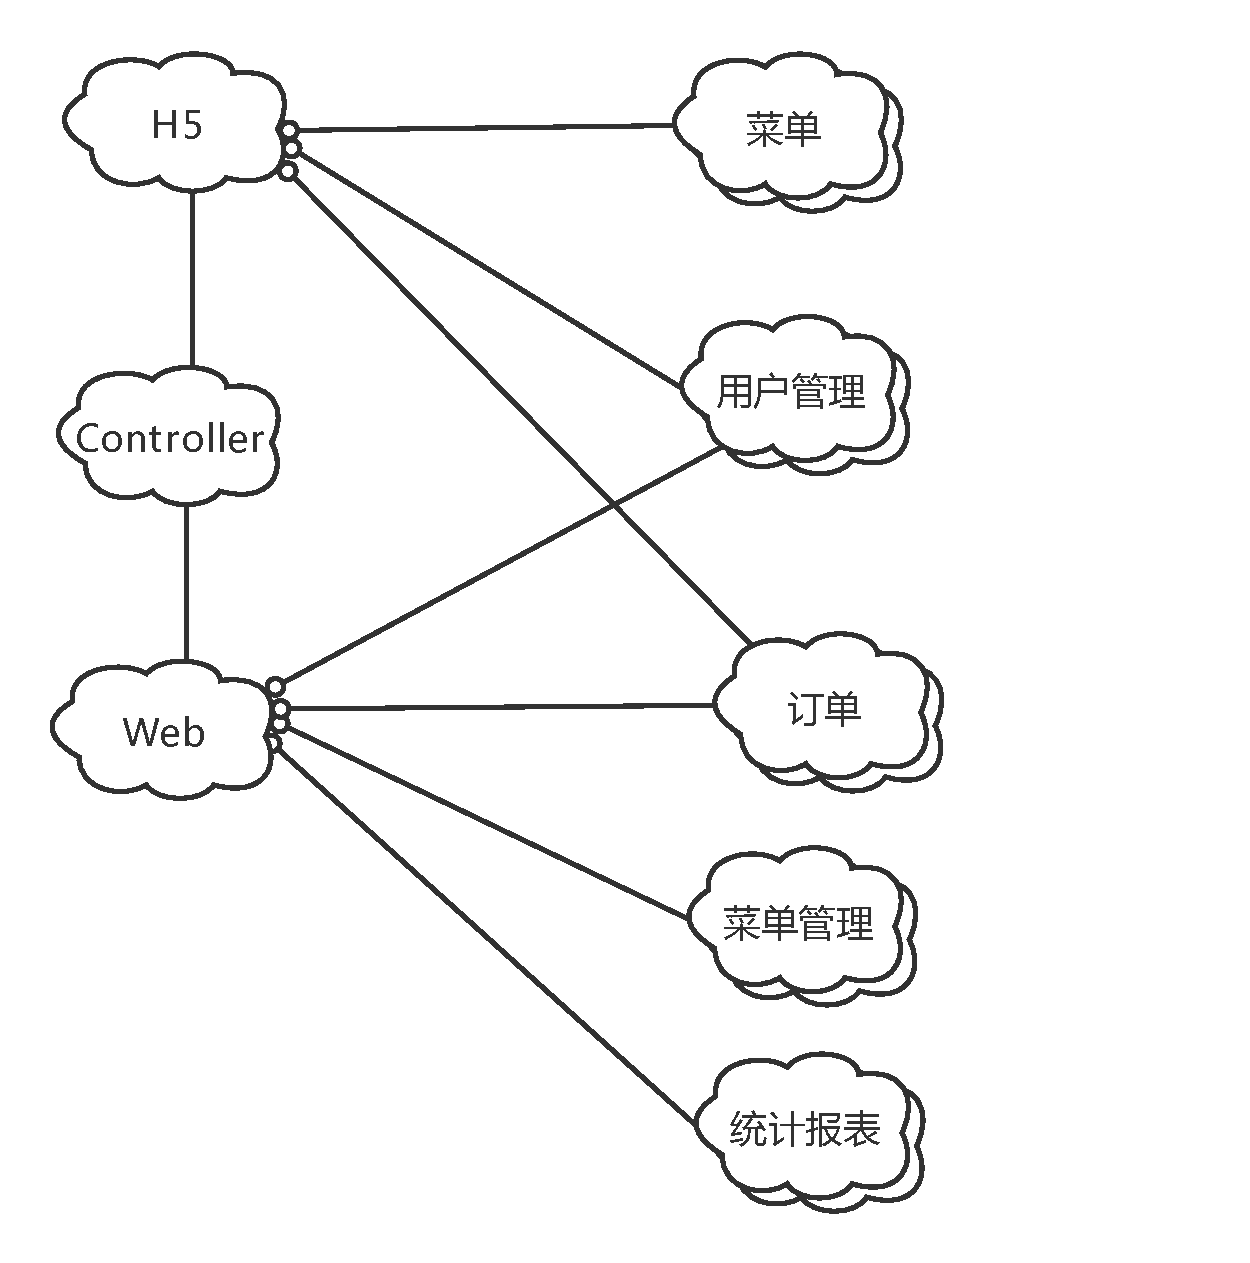
\includegraphics[width=3in]{FIGs/chapter3/logic.pdf}
  \caption{彭庆福点单系统逻辑视图}\label{fig_logicCH3}
\end{figure}

\begin{figure}[htbp!]
  \centering
  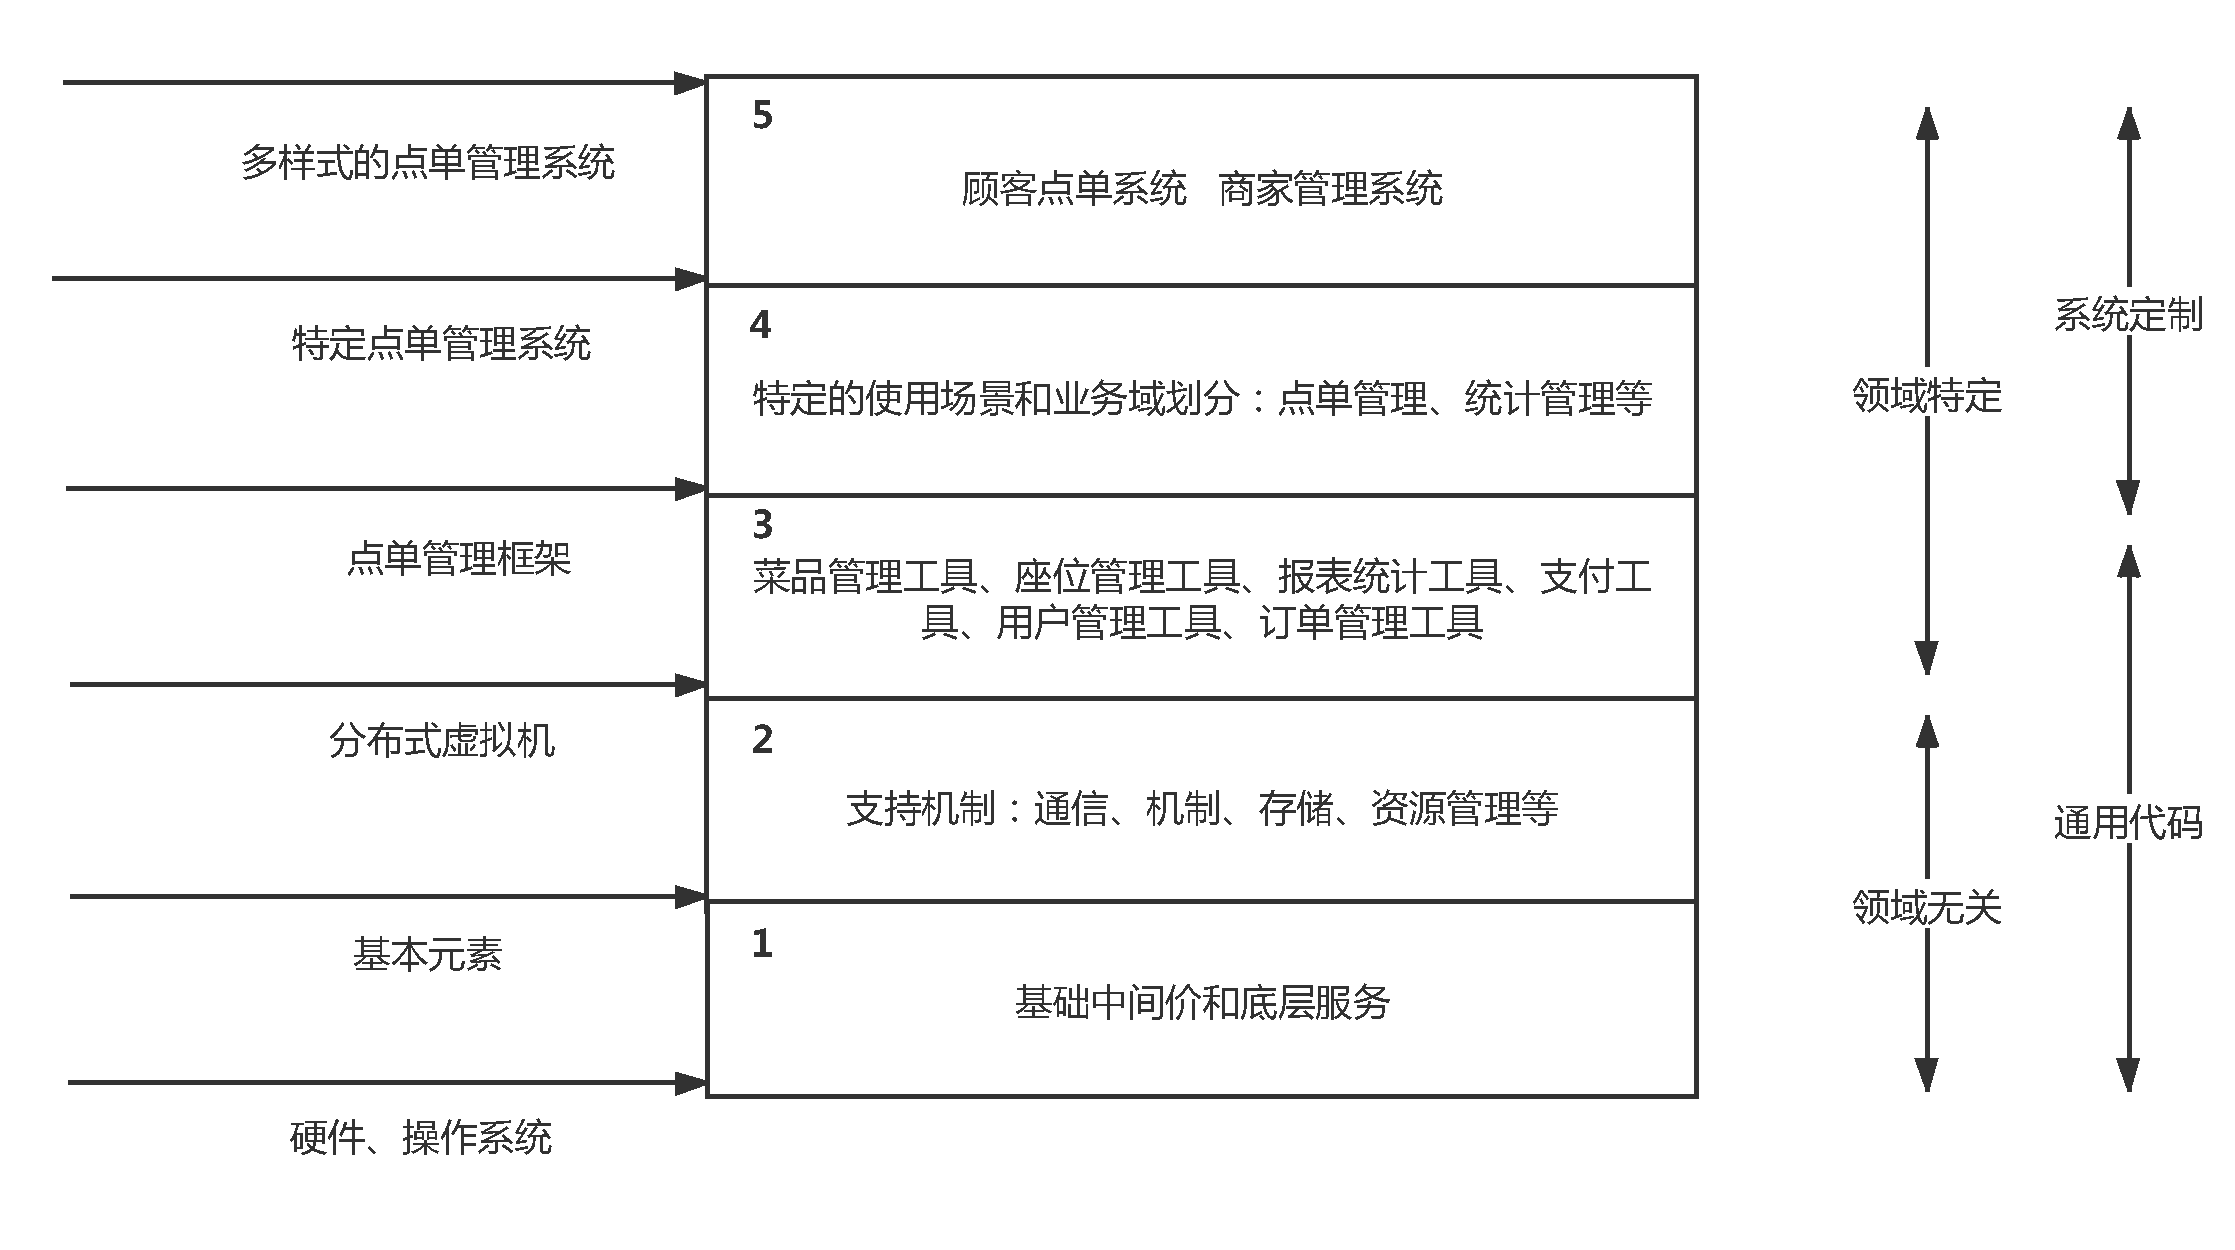
\includegraphics[width=5in]{FIGs/chapter3/develop.pdf}
  \caption{彭庆福点单系统开发视图}\label{fig_developCH3}
\end{figure}

彭庆福点单系统产品线的5个分层开发的组织结构如图~\ref{fig_developCH3}所示,系统的一二层组成了独立的、覆盖整个产品线的基础设施;第三层为基础设施增加了点单管理框架,组成了特定领域的软件架构形式;在此基础上,第四层构建了特定场景域选择,基本涵盖了系统所需功能;第五层依赖于用户和产品内容,包含了功能齐全的用户接口、外部系统接口等。

\begin{figure}[htb]
  \centering
  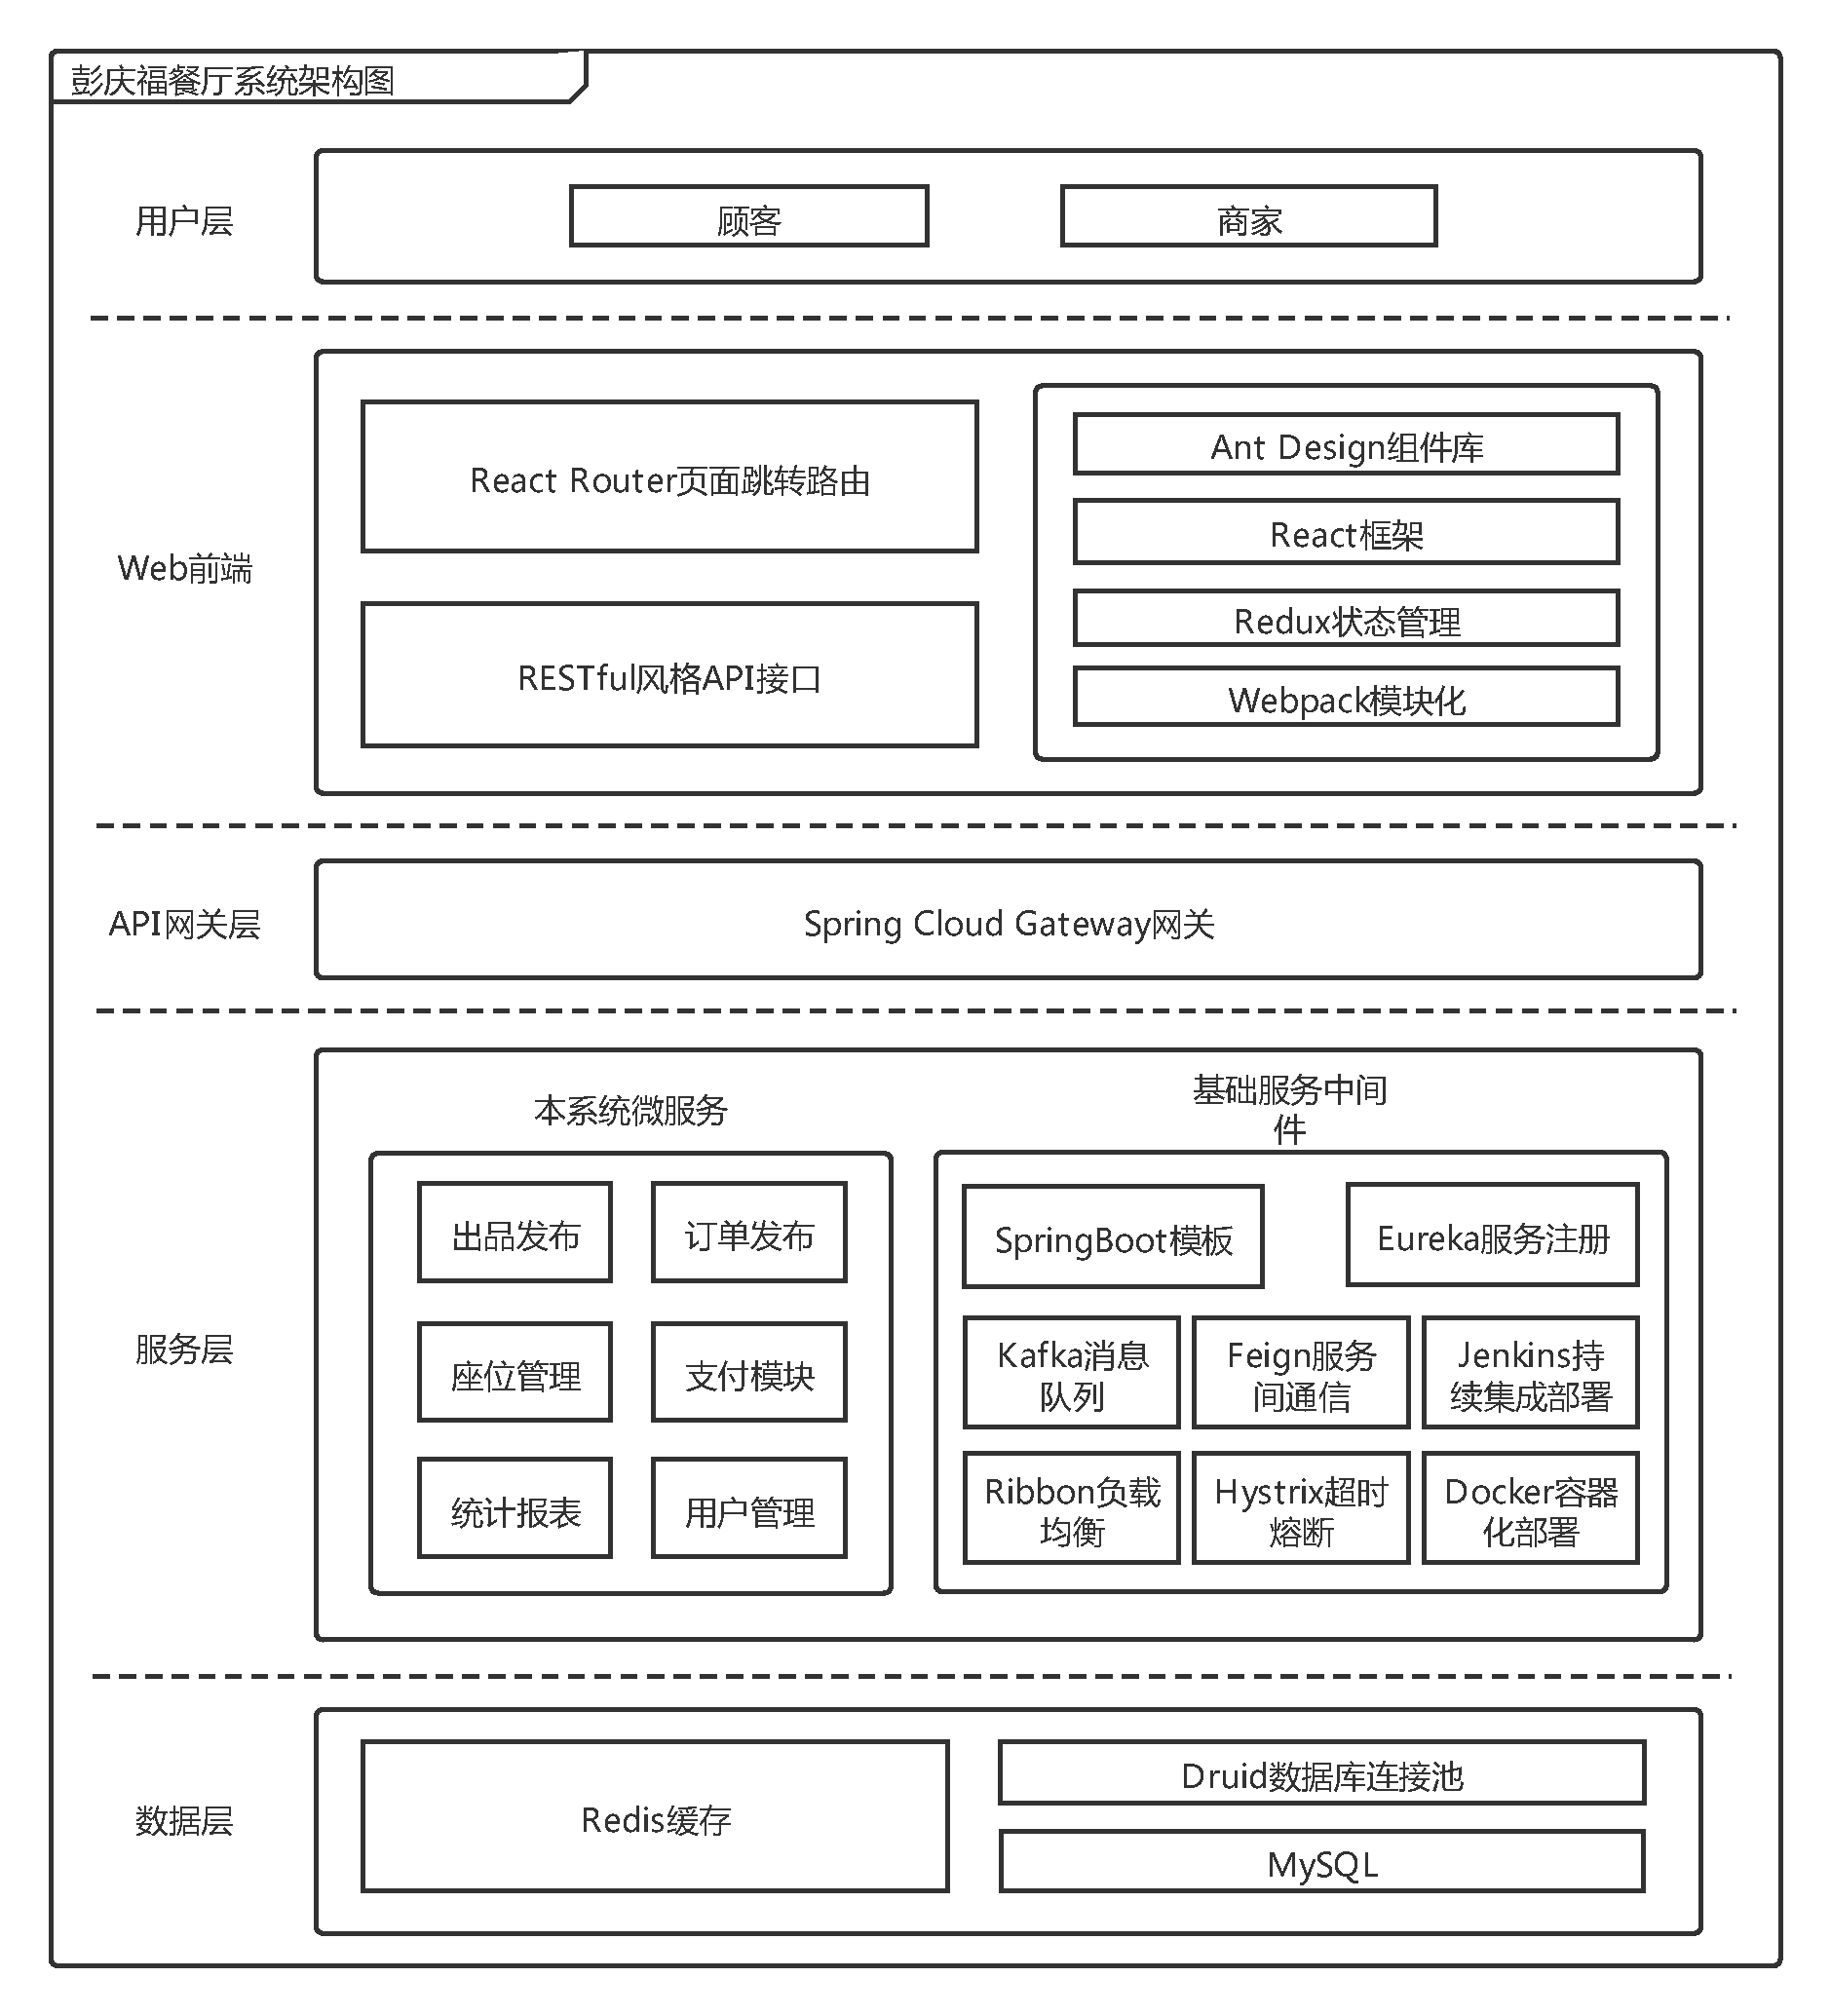
\includegraphics[width=5in]{FIGs/chapter3/all.pdf}
  \caption{系统架构图}\label{fig_allCH3}
\end{figure}

如图~\ref{fig_allCH3}所示的彭庆福餐厅点单系统架构图,系统一共可以分为用户层、Web前端、API网管层、服务层和数据层。在用户层中,考虑到顾客和商家的不同使用习惯,点单部分和管理部分分别设计成了手机浏览(H5界面)和PC端网页浏览的形式。Web前端项目由React框架搭建,可以快速渲染、局部刷新,搭配Redux技术进行第三方通信,通过把数据存储在Store里,达到状态、数据流的统一管理。页面跳转路由使用了React Router实现,并使用RESTful风格的API接口,使用了Ant Design组件库antd使得UI界面统一、美观,使用Webpack作为前端打包工具,把资源统一打包成少量文件,并结合插件进行语法转换。

API网关层负责接收Web前端发来的接口请求,使用了Spring Cloud Gateway网关,向下调用服务层提供的请求来响应,并将处理后的请求结果返还给前端~\cite{lhf2013mvc}。服务层是由一些基础服务中间件和本系统功能拆分的微服务所组成,包括出品发布服务、订单发布服务、座位管理服务、支付模块服务、统计报表服务和用户管理服务,每个服务都具有相应的功能来对应特定接口,服务之间还存在着不同的依赖,除此之外还有一些第三方服务。

数据层主要负责数据持久化,存储着彭庆福餐厅点单系统的各类数据信息,包括顾客、订单详情、菜品、订单、计划、座位、商家等信息。\\

\subsection{部署架构}
\begin{figure}[htbp!]
  \centering
  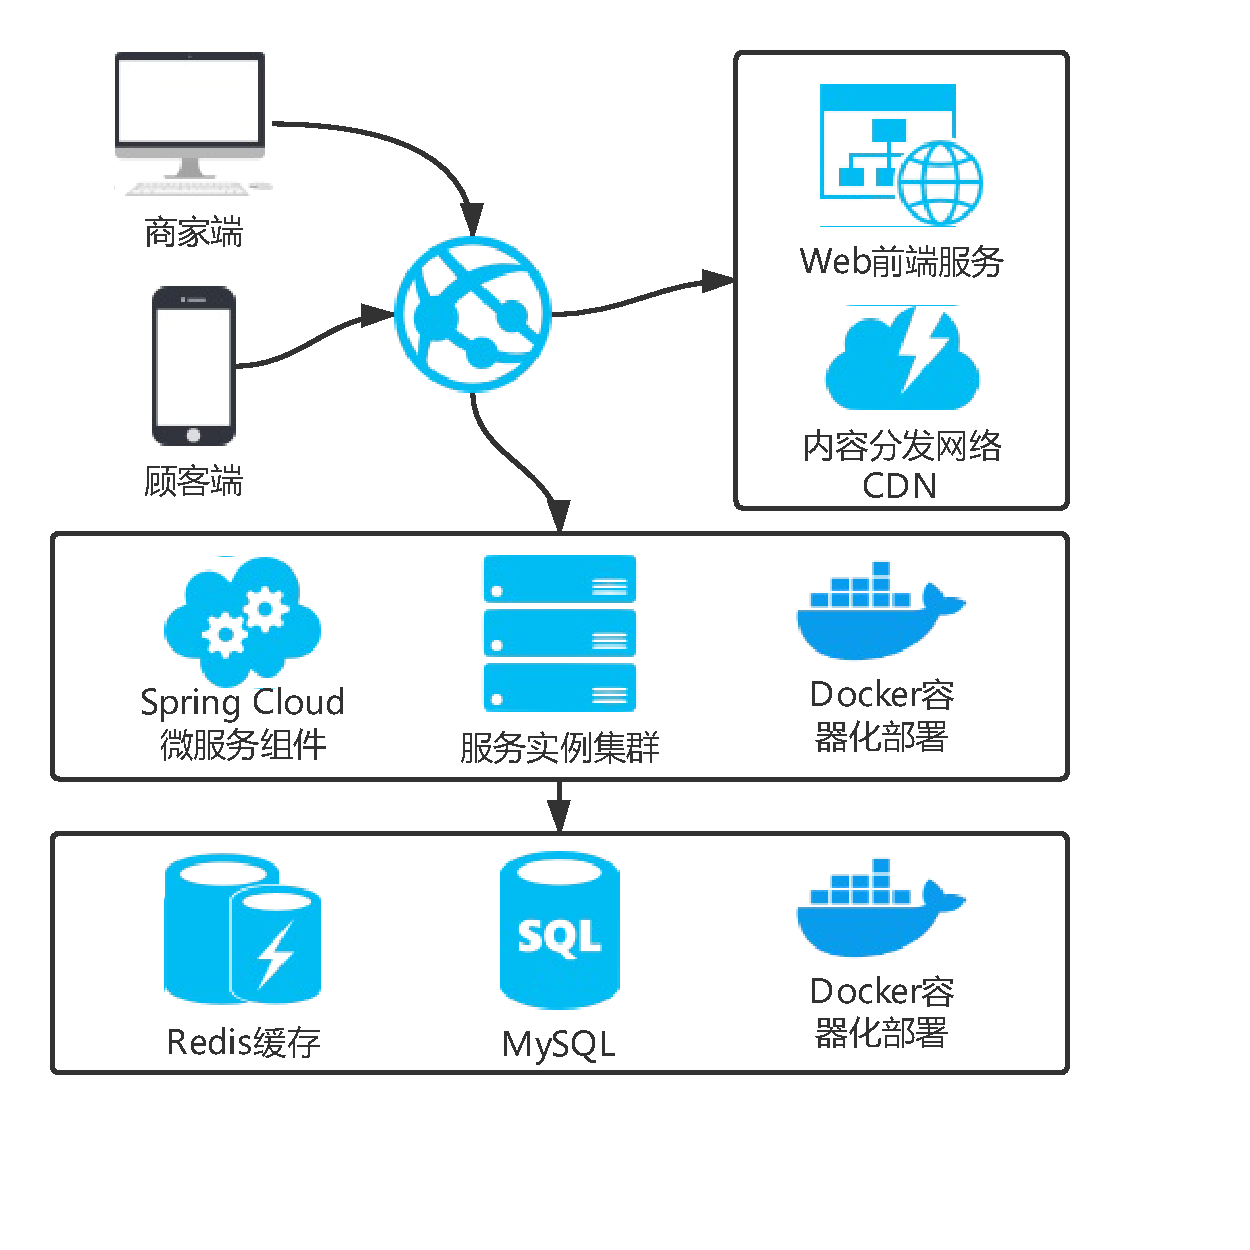
\includegraphics[width=4.5in]{FIGs/chapter3/physics.pdf}
  \caption{彭庆福餐厅点单系统物理视图}\label{fig_physicsCH3}
\end{figure}

彭庆福餐厅点单系统的部署结构主要分为三个部分:Web前端服务层、后端微服务层、数据库层~\cite{syp2018},如图~\ref{fig_physicsCH3}所示。

商家端或顾客端设备获取Web前端资源,请求会发送到Web前端服务层,这一层处理所有前端的脚本与静态资源。本层部署时首先从持续集成系统CI获取构建完整的部署包,用该部署包分组刷新服务实例,其他静态资源上传到内容分发网络CDN。

同样商家端或顾客端设备访问后端数据,请求会发到后端微服务层,这一层处理所有RESTful动态数据请求。本层部署时同样会先从持续集成系统CI获取构建完整的部署包后分组刷新服务实例,在刷新时需要先更新Spring Cloud微服务组件再更新具体业务逻辑服务。在部署组件服务和业务逻辑服务时,统一使用Docker进行容器化部署。

后端微服务层在处理请求时,访问数据库的请求会发到数据库层,这一层主要做持久化数据的存储和访问,使用缓存提高访问效率。本层部署对象包括MySQL关系型数据库和基于Redis的缓存服务,部署时二者都使用Docker的官方镜像。此外,Redis部署时需要对缓存做预热操作~\cite{wxl}。

\section{数据库设计}
\begin{figure}[htbp!]
  \centering
  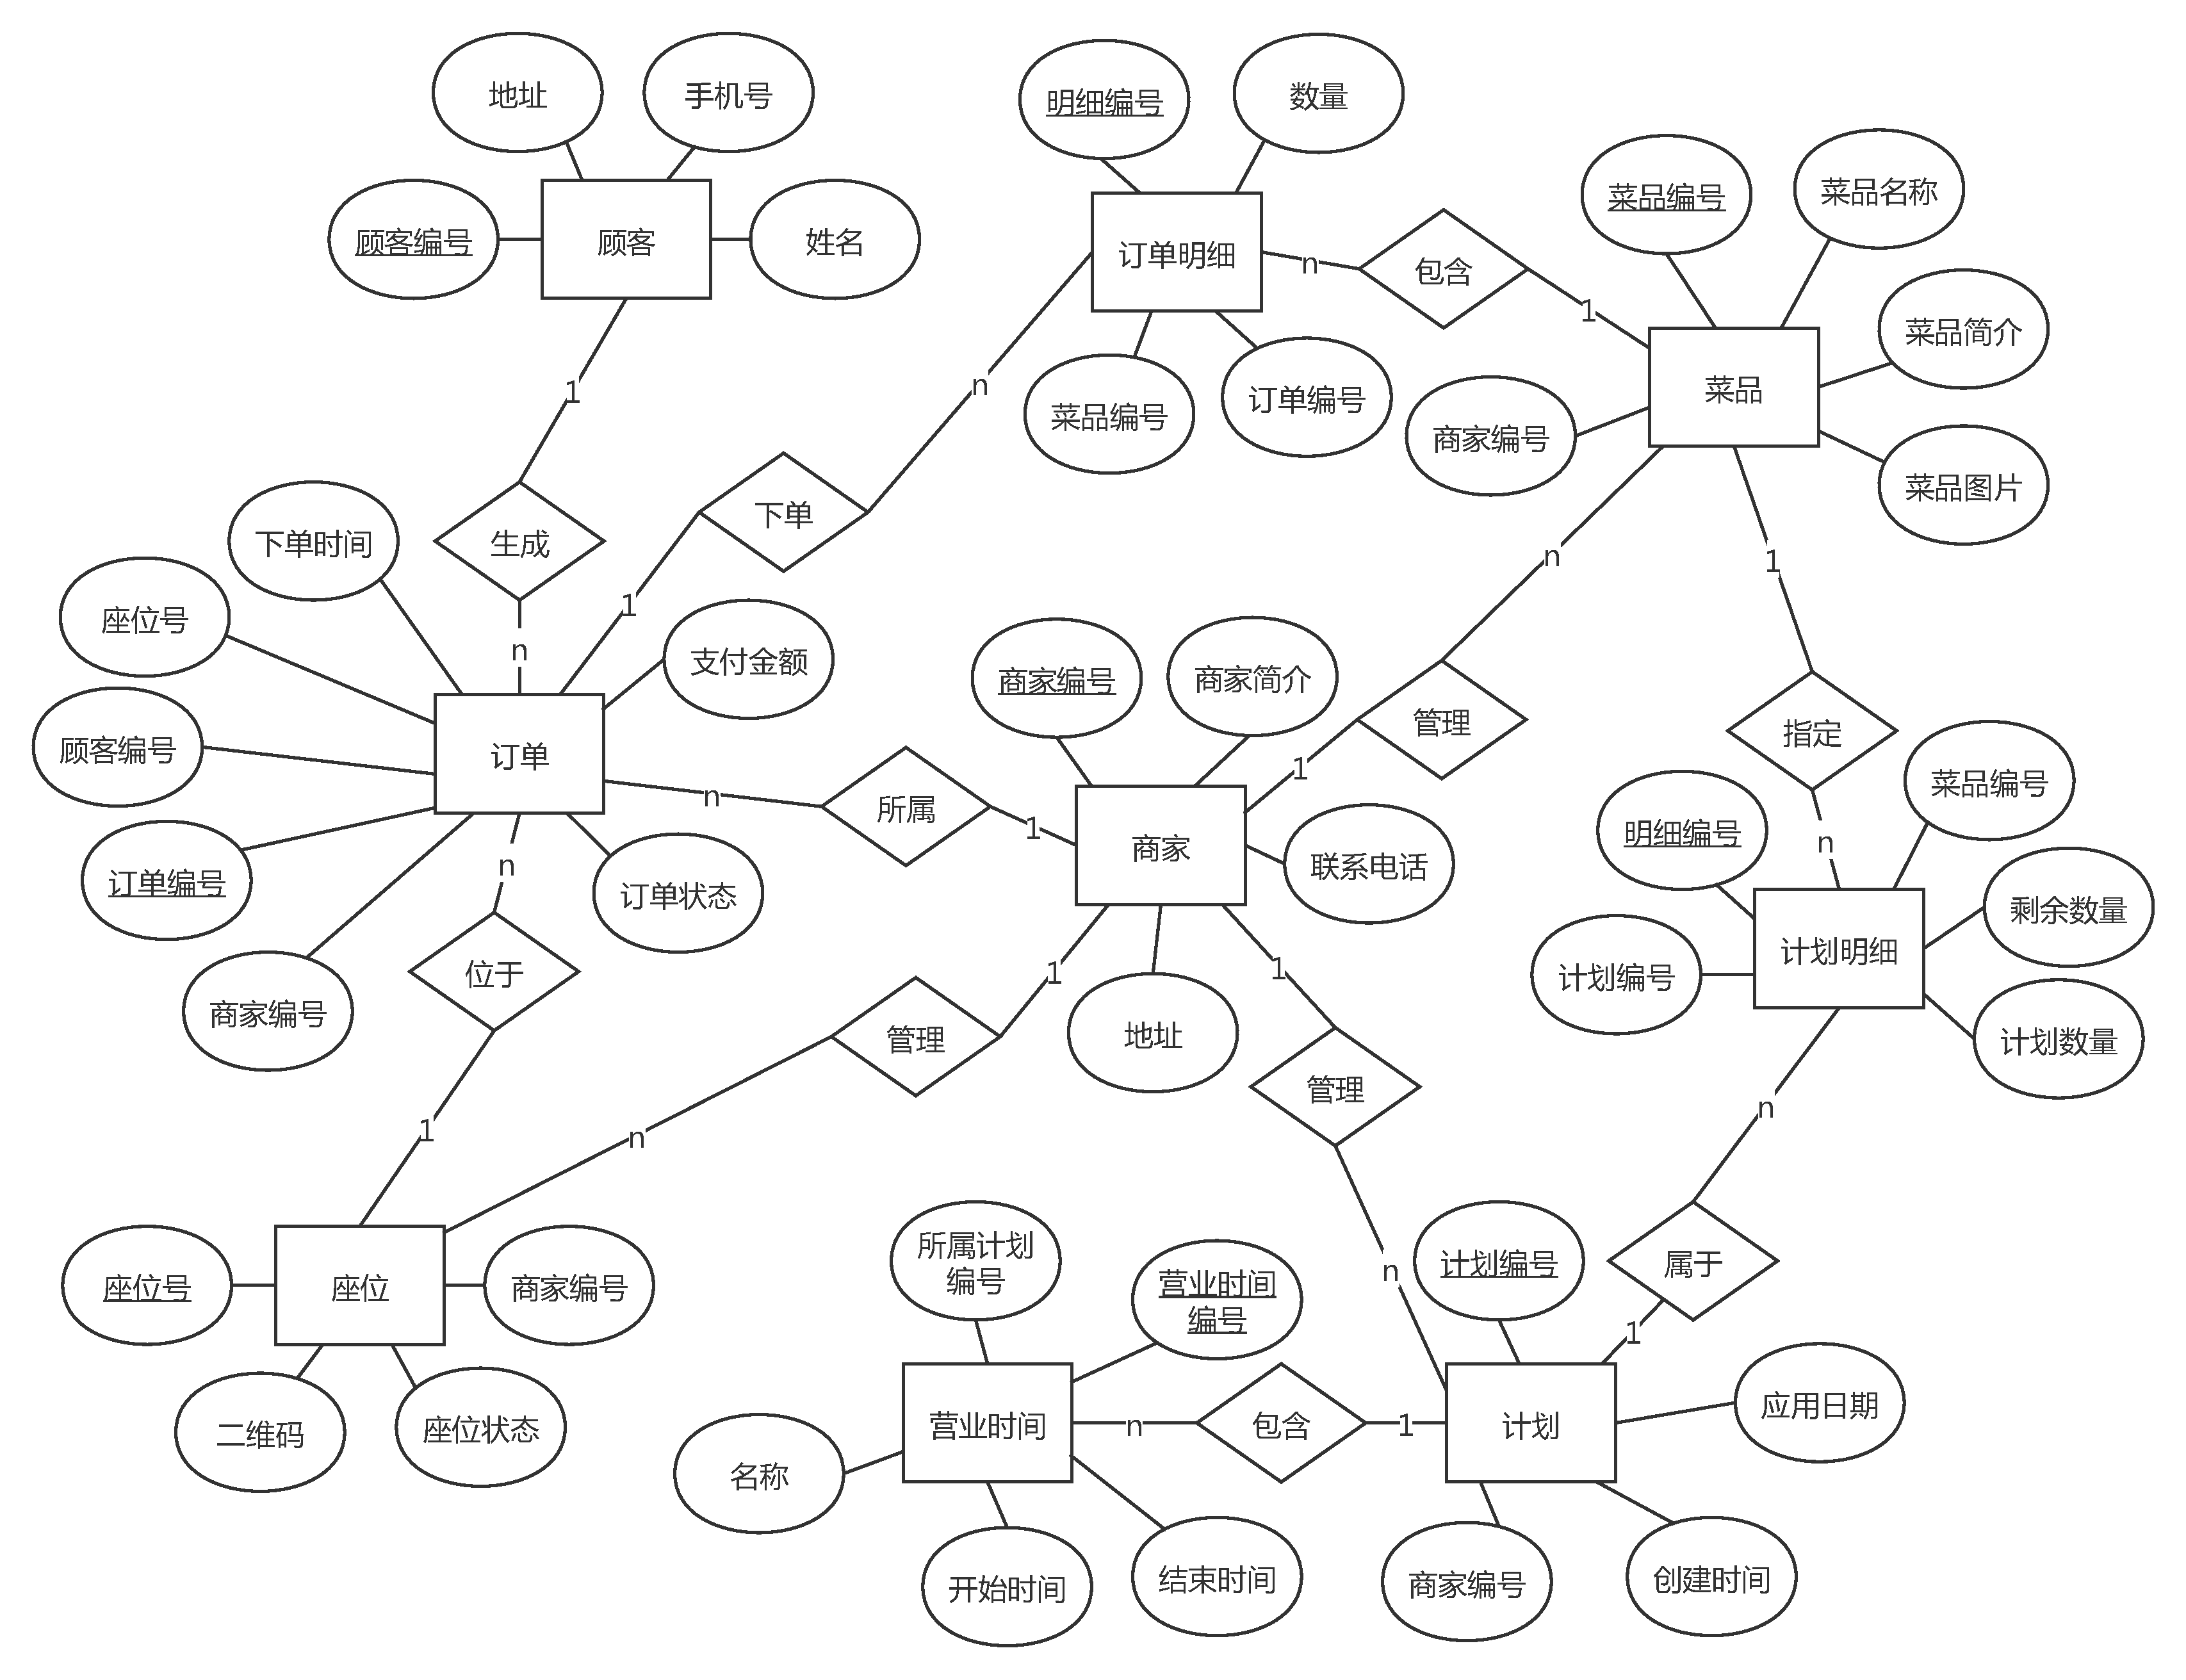
\includegraphics[width=5in]{FIGs/chapter3/ER.pdf}
  \caption{彭庆福餐厅实体关系图}\label{fig_ERCH3}
\end{figure}

结合系统的模块设计与业务需求,本项目将数据库表大致分成了四个部分,分别是订单、菜品、计划以及用户信息。

彭庆福餐厅点单系统的数据库实体关系图如图~\ref{fig_ERCH3}所示,包括顾客、商家、订单、订单详情、座位、菜品、计划、计划明细、营业时间等几个实体,实体之间存在一对多的关系~\cite{xjfMySQL}。

\begin{table}[htbp!]\footnotesize
  \centering
  \caption{顾客实体数据库表Customer}
  \vspace{2mm}
  \begin{tabular}{lllll}
  \toprule
  \textbf{名称}&\textbf{类型}&\textbf{长度}&\textbf{允许空值}&\textbf{描述}\\
  \midrule 
  customerId& bigint& 30& No& 顾客编号\\
  \hline
  name& varchar& 30& No& 顾客姓名\\
  \hline
  phone& varchar& 20& Yes& 联系手机号码\\
  \hline
  address& varchar& 50& Yes& 配送地址\\
  \bottomrule
  \end{tabular}
  \label{table:ER1}
\end{table}

顾客实体是对所有就餐客人的抽象,主要保存用户编号、姓名、手机号、配送地址等属性。
表~\ref{table:ER1}是描述顾客实体的数据库表Customer,主键为顾客编号customerId,主要记录顾客的个人信息,方便顾客下单。为提高查询效率,在主键上建立索引。

\begin{table}[htbp!]\footnotesize
  \centering
  \caption{商家实体数据库表Merchant}
  \vspace{2mm}
  \begin{tabular}{lllll}
  \toprule
  \textbf{名称}&\textbf{类型}&\textbf{长度}&\textbf{允许空值}&\textbf{描述}\\
  \midrule 
  merchantId& bigint& 30& No& 商家编号\\
  \hline
  introduction& varchar& 200& No& 商家简介\\
  \hline
  phone& varchar& 20& No& 联系电话\\
  \hline
  address& varchar& 50& Yes& 店面地址\\
  \bottomrule
  \end{tabular}
  \label{table:ER2}
\end{table}

商家实体用于描述餐厅的线下实体店,主要保存商家编号、商家简介、地址和联系电话等属性。
表~\ref{table:ER2}是描述商家实体的数据库表Merchant,主键为商家编号merchantId。为提高查询效率,在主键上建立索引。

\begin{table}[htbp!]\footnotesize
  \centering
  \caption{座位实体数据库表Seat}
  \vspace{2mm}
  \begin{tabular}{lllll}
  \toprule
  \textbf{名称}&\textbf{类型}&\textbf{长度}&\textbf{允许空值}&\textbf{描述}\\
  \midrule 
  seatId& bigint& 30& No& 座位号\\
  \hline
  merchantId& bigint& 30& No& 所属商家编号\\
  \hline
  qrcode& varchar& 20000& No& 二维码\\
  \hline
  state& int& 5& No& 座位状态\\
  \bottomrule
  \end{tabular}
  \label{table:ER3}
\end{table}

座位实体是对可用座位的抽象,主要保存座位号、二维码、座位状态和所属商家编号等属性。
表~\ref{table:ER3}是描述座位实体的数据库表Seat,主键为座位号seatId。为提高查询效率,在主键和所属商家编号上分别建立索引。

\begin{table}[htbp!]\footnotesize
  \centering
  \caption{菜品实体数据库表Product}
  \vspace{2mm}
  \begin{tabular}{lllll}
  \toprule
  \textbf{名称}&\textbf{类型}&\textbf{长度}&\textbf{允许空值}&\textbf{描述}\\
  \midrule 
  productId& bigint& 30& No& 菜品编号\\
  \hline
  merchantId& bigint& 30& No& 所属商家编号\\
  \hline
  name& varchar& 20& No& 菜品名称\\
  \hline
  introduction& varchar& 200& Yes& 菜品简介\\
  \hline
  image& varchar& 20000& Yes& 菜品图片\\
  \bottomrule
  \end{tabular}
  \label{table:ER4}
\end{table}

菜品实体是对菜单上可选菜品的抽象,主要保存菜品编号、菜品简介、菜品图片和所属商家编号等属性。
表~\ref{table:ER4}是描述菜品实体的数据库表Product,主键为菜品编号productId。为提高查询效率,在主键和所属商家编号上分别建立索引。

\begin{table}[htbp!]\footnotesize
  \centering
  \caption{订单实体数据库表Order}
  \vspace{2mm}
  \begin{tabular}{lllll}
  \toprule
  \textbf{名称}&\textbf{类型}&\textbf{长度}&\textbf{允许空值}&\textbf{描述}\\
  \midrule 
  orderId& bigint& 30& No& 订单编号\\
  \hline
  seatId& bigint& 30& No& 就餐座位号\\
  \hline
  merchantId& bigint& 30& No& 所属商家编号\\
  \hline
  customerId& bigint& 30& No& 下单顾客编号\\
  \hline
  createdAt& timestamp& 100& No& 创建时间\\
  \hline
  state& int& 5& No& 订单状态\\
  \hline
  price& float& 10& No& 支付金额\\
  \bottomrule
  \end{tabular}
  \label{table:ER5}
\end{table}

订单实体是对客户顾客就餐产生订单的抽象,主要保存订单编号、订单状态、下单时间、支付金额、所属商家编号、来源顾客编号、就餐座位号等属性。
表~\ref{table:ER5}是描述订单实体的数据库表Order,主键为orderId。为提高查询效率,在主键、所属商家编号和下单客户编号上分别建立索引。

\begin{table}[htbp!]\footnotesize
  \centering
  \caption{订单明细实体数据库表OrderItem}
  \vspace{2mm}
  \begin{tabular}{lllll}
  \toprule
  \textbf{名称}&\textbf{类型}&\textbf{长度}&\textbf{允许空值}&\textbf{描述}\\
  \midrule 
  orderItemId& bigint& 30& No& 订单明细编号\\
  \hline
  orderId& bigint& 30& No& 所属订单编号\\
  \hline
  productId& bigint& 30& No& 下单菜品编号\\
  \hline
  quantity& int& 10& No& 下单数量\\
  \bottomrule
  \end{tabular}
  \label{table:ER6}
\end{table}

订单明细实体是对订单中选择的菜品进行抽象,主要保存所属订单编号、选择的菜品编号和数量等属性。
表~\ref{table:ER6}是描述订单明细实体的数据库表OrderItem,主键为orderItemId。为提高查询效率,在主键和所属订单编号上分别建立索引。

\begin{table}[htbp!]\footnotesize
  \centering
  \caption{计划实体数据库表Plan}
  \vspace{2mm}
  \begin{tabular}{lllll}
  \toprule
  \textbf{名称}&\textbf{类型}&\textbf{长度}&\textbf{允许空值}&\textbf{描述}\\
  \midrule 
  planId& bigint& 30& No& 编号\\
  \hline
  merchantId& bigint& 30& No& 所属商家编号\\
  \hline
  createTime& timestamp& 100& No& 创建时间\\
  \hline
  applyDate& date& 50& No& 应用日期\\
  \bottomrule
  \end{tabular}
  \label{table:ER7}
\end{table}

计划实体用于描述商家对菜品销售和营业时间的计划,主要保存计划编号、所属商家编号、创建时间和应用日期。
表~\ref{table:ER7}是描述计划实体的数据库表Plan,主键为计划编号planId,是出品计划的实体内容,需要与计划明细实体、营业时间实体相关联,从而为每个出品计划绑定菜单、库存数、计划数以及餐厅当日营业时间等内容。为提高查询效率,在主键和所属商家编号上分别建立索引。

\begin{table}[htbp!]\footnotesize
  \centering
  \caption{计划明细实体数据库表PlanItem}
  \vspace{2mm}
  \begin{tabular}{lllll}
  \toprule
  \textbf{名称}&\textbf{类型}&\textbf{长度}&\textbf{允许空值}&\textbf{描述}\\
  \midrule 
  planItemId& bigint& 30& No& 编号\\
  \hline
  planId& bigint& 30& No& 所属计划编号\\
  \hline
  productId& bigint& 30& No& 指定菜品编号\\
  \hline
  quantity& int& 10& No& 计划数量\\
  \hline
  remain& int& 10& No& 剩余数量\\
  \bottomrule
  \end{tabular}
  \label{table:ER8}
\end{table}

计划明细实体是指计划中包含的单个菜品销售计划,包括计划明细编号、所属计划编号、指定菜品编号、计划数量和剩余数量等属性。
表~\ref{table:ER8}是描述计划明细实体的数据库表PlanItem,主键为计划明细编号planItemId。为提高查询效率,在主键和所属计划编号上分别建立索引。

\begin{table}[htbp!]\footnotesize
  \centering
  \caption{营业时间实体数据库表PlanSlot}
  \vspace{2mm}
  \begin{tabular}{lllll}
  \toprule
  \textbf{名称}&\textbf{类型}&\textbf{长度}&\textbf{允许空值}&\textbf{描述}\\
  \midrule 
  planSlotId& bigint& 30& No& 编号\\
  \hline
  planId& bigint& 30& No& 所属计划编号\\
  \hline
  name& bigint& 30& No& 时间段名称\\
  \hline
  startTime& timestamp& 100& No& 开始时间\\
  \hline
  endTime& timestamp& 100& No& 结束时间\\
  \bottomrule
  \end{tabular}
  \label{table:ER9}
\end{table}

营业时间实体是对商家当日计划营业时间的抽象,主要保存营业时间编号、所属计划编号、时间段名称、开始时间和结束时间。
表~\ref{table:ER9}是描述营业时间实体的数据库表PlanSlot,主键为营业时间段编号planSlotId。为提高查询效率,在主键和所属计划编号上分别建立索引。

订单实体由顾客实体生成,被商家管理,一位顾客可以生成多个订单,商家也可以拥有多个订单,所以顾客与订单、商家与订单都是一对多的关系。
订单中可能包含不同数量的多种菜品,本系统使用订单详情实体来管理这种关系,订单与订单详情、菜品与订单详情都是一对多的关系。
商家可以管理菜品列表,也可以管理每日计划安排,所以商家与菜品、商家与计划实体都是一对多的关系。每个计划是指商家当日出品计划和营业时间段安排,包含不同数量的多个菜品,还包含多个不同营业时间段,因此计划实体与计划明细、计划实体与营业时间是一对多的关系~\cite{ssh2019}。

\section{本章小结}
本章对彭庆福餐厅点单系统的整体概要设计以及需求进行了分析。首先,对系统设计目标做了详细说明,分析其可行性,并通过系统整体结构图介绍了系统组成部分。接着,将项目需求从两个方面进行了阐述,包括功能需求——主要通过绘制用例图表对系统两类用户(顾客和商家)的需求进行了归纳,以及非功能需求——从可用性、系统性能、支持性、可靠性以及安全性进行了分析。并分析了较为重要的顾客功能执行的流程设计,从逻辑视图、开发视图、系统架构图等分析了系统模块交互,介绍了总体的架构设计和部署架构。通过实体关系图解释了系统的数据库设计,并对数据库表内容做了简要分析。